\documentclass[a4paper, 12pt]{article}
\usepackage{newtxtext,newtxmath}


\usepackage{geometry} % Простой способ задавать поля
\geometry{top=25mm}
\geometry{bottom=25mm}
\geometry{left=30mm}
\geometry{right=20mm}
\usepackage{multirow}
\usepackage{cmap}                
\usepackage{mathtext} 
\usepackage{adjustbox}
\usepackage[T2A]{fontenc}
\usepackage[utf8]{inputenc}    
\usepackage[british]{babel}	
\usepackage{rotating}
\usepackage{float}

\usepackage{tablefootnote}
\usepackage{threeparttable}
\usepackage{threeparttablex}
\usepackage{setspace}
\usepackage{amsmath}
\usepackage{tikz}
\usetikzlibrary{shapes.geometric}
\usepackage{amssymb}
\usepackage{bm}
\usepackage{pifont}% http://ctan.org/pkg/pifont
\newcommand{\cmark}{\ding{51}}%
\newcommand{\xmark}{\ding{55}}

%\usepackage[paper=portrait,pagesize]{typearea}
\usepackage{subfig}


%\usepackage{euscript}     % Шрифт Евклид
%\usepackage{mathrsfs} % Красивый
%матшрифт
\onehalfspacing
\usepackage{lscape}

%%% Работа с картинками
\usepackage{graphicx}  % Для вставки
%рисунков
\graphicspath{img/}  %
%папки с картинками
\setlength\fboxsep{3pt} % Отступ рамки
%\fbox{} от рисунка
\setlength\fboxrule{1pt} % Толщина линий
%рамки \fbox{}
%\usepackage{wrapfig} % Обтекание
%рисунков и таблиц текстом
\usepackage{grffile}

\usepackage{csquotes}
\usepackage[style=apa, sorting=nty, bibencoding=utf8]{biblatex}
\addbibresource{citations.bib}
\DeclareLanguageMapping{british}{british-apa}

\usepackage{hyperref}


\title{%
Land titling and industrial development\\
\Large Case of the Stolypin reform}
\author{Vladimir Novikov \& Igor Kolesnikov}
\date{Fall 2021}

\begin{document}

%\vspace{5cm}
\maketitle

\noindent VERSION FOR JANUARY 2022

\subsection*{Abstract}

\textit{We study the effect of the land titling on industrial development, using the case of the Stolypin reform in Late Imperial Russia. We make use of the unique city-level dataset to estimate the effect of the reform implementation on industrialization as such, industrial productivity and factories size. During the first years of the reform, it procreated a major labor shock with ambivalent direct and spillover effects on industrial development.}

\newpage

\section{Introduction}


In recent years, the interest in economic development of Imperial Russia was surging \parencite{gur2021}. Some of the papers focus on regional variation \parencite{markevich2019regional}, while others trace long-term trends \parencite{markevich2018economic, markevich2011great}. Among other research subjects, the Stolypin agricultural reform stands apart. Recently, its effect on internal migration and agricultural productivity was detailed \parencite{chernina2014property, castaneda2019stolypin}. Since the reform enhanced the liquidity of land assets and reduced some of the costs peasants had to bear,  it dramatically reshaped the economic life of Russia, despite falling short of the initial goals of the policy. However, there are still some gaps in our understanding of the reform and its aftereffects. For instance, we still do not have a definitive account of migration this reform facilitated, since only the migration to the East was rigorously studied. When it comes to the migration itself, there is a lack of knowledge regarding its role in industrial development and transformation of the imperial economy at the beginning of the XX century. 
\\\\
This paper will try to address those gaps in our understanding of the reform, but also fit into somewhat broader theoretical questions. There is already some evidence that land consolidations and village-wide abolition of communes facilitated technological development in the agricultural sector \parencite{castaneda2019stolypin}. Some accounts lay the ground for the fact that land titling can alter individual investment'.  This program of land titling started in 1907 allows studying how similar programs can change an individual choice of one's occupation and, therefore, the structure of the labor market. As we will discuss in the theoretical section, the effect of the reform should be especially sound because it was peasants who were the major source of labor for the industrial sector at that time in the empire. Therefore, their calculations with regard to job opportunities should have affected resources available to businesses at that stage of industrial development.
\\\\
Further on, we will make the case that the progress of the Stolypin was associated with significant transformation in cities' labor market, which in turn affected the industrial development of Late Imperial Russia. Our research question is \textbf{how land titling for peasants affected urban industrial development in Late Imperial Russia?}
\\\\
In general, the reform implementation procured two major effects in terms of industrial development and labor market. First of all, it gave incentives to peasants leaving their part-time seasonal work at a factory and focusing solely focus on the development of their individually owned parcel of land. In contrast, the reform also created a spillover effect, facilitating the wave of internal migration within adjacent provinces from villages to cities. Both of those effects were associated with changes in the number of workers employed in cities and number of factories. However, the lack of data on industrial development after 1910 prohibits exploring long-term effects of the reform, including productivity per worker and other parameters. 


    
    %некоторое множество общих слов и problem statement
    
\section{Literature}    
    
    %здесь литература про property rights & economic outcomes in general
    %и немного конкретики про влияние конкретно land titlting на миграцию, а миграции (в города) и вообще урбанизации на индустриализацию 
    
    
In this section, we lay out previous findings regarding the relationship between similar programs of land titling and internal migration. Moreover, insights from literature about  the question how such migration later affects industrialization will also be provided. 
\\\\
There are several main channels through which land titling have a positive effect on the internal migration of farmers and peasants. First of all, receiving property rights for land secure the land plot for the peasant and make it much more protected \parencite{field2007entitled}. Because of this, the previous resource costs (including time costs) needed to preserve the land are significantly reduced, and the farmer gains more employment opportunities in urban areas with a predominance of industrial sectors of the economy. In addition, the risks associated with the expropriation of land titles are also reduced for the peasant  \parencite{aragon2020property}. Therefore, she is more likely to leave her allotment and work in the non-agricultural sector within the city. The second explanatory mechanism is the easing of the liquidity constraint \parencite{cai2020migration} - the granting of title to land allows peasants to freely sell or lease their plots. Thus, they can manage land more efficiently by developing a market for agricultural land and reducing transaction costs, which creates additional incentives for migration from rural areas. De Janvry  also showed, using the 1993-2006 Mexican land certification programs, that the issuance of land title deeds increases the likelihood of a household member migrating by 28\% \parencite{de2015delinking}.
\\\\
An alternative view among researchers is that giving farmers rights to their land plots, on the contrary, leads to a limitation of internal migration in the country. If a farmer obtains property rights, she is more incentivized to invest in her land, as the marginal benefits of her upkeep will increase under a restrained redistributive government policy \parencite{hong2020land}. At the same time, the opportunity cost of migration to the city increases for the farmer, which forces him to stay in rural areas. In addition, there is an indirect endowment effect - the willingness to take ownership of the land is higher than the willingness to pay for it \parencite{kahneman1991anomalies}. In the absence of an adequate willingness to pay on the demand side, this effect can lead to a reduction in land transactions and hinder internal migration of peasants. In China, it was detailed that there is no significant direct impact of land ownership on peasant migration to cities \parencite{li2021land}. This finding indicates that other factors, such as wage differentials between the agricultural and industrial sectors, may also influence migration from rural to urban areas.
\\\\
The second part of the research, which is necessary to understand the essence of this work, focuses on assessing the effect of migration of rural workers on urban productivity. The idea of the mechanism is that the inflow of human capital into cities increases the level of technology and the productivity of industrial enterprises. This connection is confirmed in a number of works. The results of another  study  show that the growth of a city's size has a positive effect on its productivity\parencite{shen2019city}. This mechanism is consistent with the results of earlier research on “agglomeration economies” in cities in developing countries. Da Mata concluded that declining agricultural incomes contributed to the growth of Brazilian cities in the 1970s and 2000s both in terms of population and production values \parencite{da2005determinants}. Urbanization and concentration of the workforce in cities lead to positive externalities for adjacent enterprises and territories, which creates favorable conditions for new labor migrants and competing firms.
\\\\
On the other hand, the link between rural-to-urban migration (urbanization) and productivity growth is not so straightforward. Turok and McGranahan analyzing cities in developing countries note that rapid urbanization does not directly determine economic growth, but only contributes to it in a steady state, when there is no problem with “absorbing surplus urban labor” \parencite{turok2013urbanization}. Most current research also emphasizes the temporary nature of productivity gains, as high concentration of population in urban areas and the effect of technology spillovers at some point begin to slow such growth \parencite{bertinelli2004urbanization, lee2015agglomeration } .

    
    
\section{Historical context}


% Тут надо достаточно подробно написать про процесс реформы: выходы и консолидации двух видов + про общину и мотивацию реформы + про то что реформа поменялась в 1910 году

%И про индустриальное развитие РИ    

In 1906, the key policy of Pyotr Stolypin took place -- the agrarian reform. After the Great reforms of Alexander II, striped and distant lands emerged because plots of communes were mixed with plots of private landowners. The overlap led to the fact that to get to your plot, you had to pay for the passage to the landowner or go around, reducing the incentives to cultivate the land and to carry fertilizers there. The patchwork was also due to the redistributive nature of the repartition commune. Regular redistribution campaigns led to some areas being located so far away they were not cultivated at all \parencite{davydov}. These inefficiencies were reflected in aggregate figures. At the time of the reform, Russians had more land per capita than Italian, Austrian, and German peasants. Despite that, consumption per household was relatively modest (in France -- 33.6 poods per capita per year, in Russia 19.5). \cite{nefyodov}).
\\\\
Moreover, this also slowed down the industrial development: low efficiency of land cultivation led to low income. Thereby, consumption is lower, restraining the growth of domestic market \parencite{litoshenko}. What is more, the institution of commune hold back the migration of peasants to cities for permanent residence since it was necessary to obtain the consent of the descent, and the they were reluctant in giving it.
\\\\
The Stolypin reform provided incentives for peasants to either exit a commune individually or annihilate it in a collective pursuit. Generally speaking, the reform established a mechanism for the privatization of land parcels by peasants. Specifically, a peasant had two options: she could demand consolidation of her plots into a single territory in the cut with the preservation of the yard in the village or exit a commune and establish a farm with the resettlement from a village to her plot. There were two types of consolidation \parencite{castaneda2019stolypin}. The first  granted an opportunity to both swap parcels with a commune and then stand out from a commune, even if other peasants did not want to do it (hereafter singular consolidations). The second one implied village-wide redistribution of land and then its subsequent privatization. In both cases, after the transition to farms and cuts, a peasant possessed all signs of ownership. In the case of a sole exit, the peasant could demand land in one place and elimination of striped plots, opening up to one place. Separately, it should be said an individual exit from the community was under the control of the land captains. This occupation emerged ten years before the reform when the state patronized the community. Their interests and identities can potentially explain the unevenness of the reform implementation across the empire. 
\\\\
Over the course of the reform, more than 6 million applications were submitted to change the conditions of land use. Since the demand was massive, the imperial state established Land Survey Commissions only in the 33 provinces  of the European part of the Empire. At the same time, the state helped peasants, granting preferential loans for acquiring land.  The fund of the Peasant Bank itself, received from the state, amounted to 8.5\% of all state revenues \parencite{davydov}.
\\\\
Regarding industrial development, the industry was replenished not only with workers but also with peasants' waste. During winter, when there was little work in the village, the peasants often went to the cities for seasonal work to earn extra money. Only from the Central Black Earth Region, about a fifth of the able-bodied population left, and these are millions of people, however, in cases where the land deficit is less than in the Center, the work may be less due to lack of need, and somewhere more, like in Siberia, where the settlers could be more active than in other provinces\parencite{davydov}. For example, 7 million passports were issued in 1897, which is an impressive indicator of the number of migrant workers, since most of them took their passports for the sake of leaving \parencite{laktykina}. The motives of emigrants themselves could be different: land shortages, heavy direct and indirect taxes (to pay arrears), or bad harvest. In winter and spring, peasants went to work on grain and river docks, load barges, do carpentry, and others. In autumn and winter, for woolen and tanneries. Also, depending on the regions, workers might go to the gold mines.



    
\section{Theoretical mechanism \& empirical hypotheses}    
    
    \noindent Given what we know about the industry in the Russian Empire, we suppose that the Stolypin reform produced two main effects, changing the labor supply in the industrial sector. First of all, it created an opportunity for peasants to focus solely on agricultural work, instead of combining part-time work at a factory and in the agricultural sector. In our context, it means that there should have been a short-term negative labor shock within provinces, causing the shrinking of the labor force and closure of some factories around the Russian Empire.  These results are partially driven by an increase in the agricultural productivity studied in \cite{castaneda2019stolypin}.
    \\\\
    Secondly, the Stolypin reform fostered internal migration, as it studied by \cite{chernina2014property}. Alongside with Eastward migration, it also eased change of occupation and residence inside the European part of Russia  through the increased liquidity of land assets. In turn, this migration caused a relocation of the labor force to industrial centers not within provinces but within connected regions. 
\\
        
    
\begin{figure}[!htbp]
        \centering
    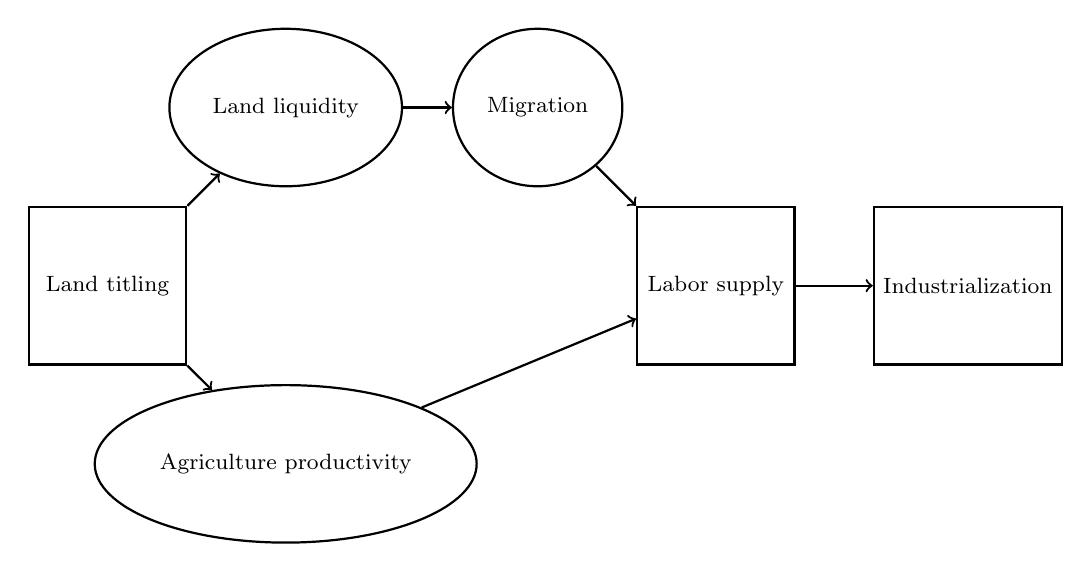
\begin{tikzpicture}[node distance={32mm}, thick, main/.style = {draw, rectangle}, lat/.style={draw,ellipse}]
\node[main,minimum size=2cm] (1) {\footnotesize{Land titling}}; 
\node[lat,minimum size=2cm] (2) [above right of=1] {\footnotesize{Land liquidity}}; 
\node[lat,minimum size=2cm] (3) [right of=2] {\footnotesize{Migration}}; 
\node[main,minimum size=2cm] (4) [below right of=3] {\footnotesize{Labor supply}};
\node[main,minimum size=2cm] (5) [right of=4] {\footnotesize{Industrialization}}; \node[lat,minimum size=2cm] (6) [below right of=1] {\footnotesize{Agriculture productivity}};

\draw[->] (1) -- (2);
\draw[->] (2) -- (3);
\draw[->] (3) -- (4);
\draw[->] (4) -- (5);
\draw[->] (6) -- (4);
\draw[->] (1) -- (6);
\end{tikzpicture}
        \caption{Expected theoretical mechanism}
        \label{fig:scheme}
    \end{figure}

% тут еще раз напишем про: права собственности -> ликвидность -> миграция -> индустриализация   


\noindent Figure \ref{fig:scheme} sumps up our expectations. Observable factors drawn in rectangles, while unobservable within our data in ellipses\footnote{While we have data on emigration in Asian provinces, we don't have any estimates of within-province migration} (precise data description is in the following section). We consider land titling having a two-fold effect on industrialization. First, it allowed peasants to leave their job at a factory, but it also granted an opportunity to dramatically change an individual life trajectory through extrication from a commune. Later on,  the second group who torn up their bonds with communes would become urban residents, bolstering the industrial development.  So, high rates of participation in reform had a negative effect within provinces but a positive effect within historically and infrastructurally interlinked regions (positive spillover effect).  The fact that we have different measures of the reform: individual exits from a commune and consolidation of land into privately owned parcels substantiates this interpretation even further. The negative labor shock should rise as both consolidations and exits increase, since they both cause the shrinkage of the labor force within a province. However, we expect only exits to have a  significant spillover effect because land consolidations providing peasants with land parcels caused them to stay in the communities but now as farmers. It is the exits providing only monetary compensations that increased migration between provinces. 
\\\\
\noindent Thereby, we draw the following set of hypotheses for our empirical study:
\begin{quote}
    H1: \textit{Both land consolidations and exits are associated with lower levels of industrial development within  provinces' cities}\\
    H2: \textit{Exits are associated with higher levels of industrial development in cities located outside provinces but within interlinked regions of the Russian Empire}
\end{quote}
    
\section{Data}   

    \begin{figure}[!htbp]
        \centering
        \includegraphics[width=\textwidth]{img/city_statuses.jpeg}
        \caption{Sample of cities by administrative status in European Russia (excluding Poland and Finland)}
        \label{fig:city_status}
    \end{figure}
    
    
    
    
    \noindent To resolve these objectives, we construct a unique city-level dataset for 1904 and 1910 (exit procedure changed dramatically) years. We make use of the set of both published and historical sources.  To do so, we followed several steps. First of all, we digitized 1904 and 1910 surveys of the cities in the Russian Empire. These surveys provide information about 1231 cities and villages, accommodating  $21501836$ people in 1904 and $27107122$ people in 1910. It is fair to ask whether this sample is representative of the global population of cities located in the Russian Empire? According to data from the annual collection of the imperial interior ministry, $24112260$ people were residing in cities in 1910 \parencite{internal}. So, the dataset includes information about settlements having an urban status at that time and about minor villages too. This fact can be seen when one looks at the spatial distribution of our data. Alongside provincial and uezd (county) centers, there are also some minor types of settlements including, for example, Miasteczko.
    \\
    
    \noindent For every settlement, we have identified its uezd (county) and province, which is helpful for subsequent matching with variables measured at the province and the uezd levels. While the province-level data comprises information about the reform progress and some additional controls (from 1907 to 1910), the latter is a digitized version of the 1897 census.
    \\
    
\begin{table}[!htbp]
    \centering
       \caption{The Stolypin reform, migration and provincial economic performance, city industrialization }
    \label{fig:sources_tab}
    \resizebox{\textwidth}{!}{
\begin{tabular}{ |p{6cm}|p{5cm}|p{2cm}|  }
 \hline
 Variable Name & Source& Period \\
 \hline
  \hline
 Exits, village-wide consolidations, singular consolidations  (number of households)    & \parencite{castaneda2019stolypin} &1907- 1910  \\
 \hline
 Production (Annual total production in thousand rubles)& \cite{goroda1904,goroda1910} & 1904, 1910    \\
  \hline
 Factories (Number of factories in a city) & \cite{goroda1904,goroda1910} & 1904, 1910    \\
  \hline
  Workers (Number of workers in a city)& \cite{goroda1904,goroda1910} & 1904, 1910    \\
   \hline
  City population ( Number of city residents)& \cite{goroda1904,goroda1910} & 1904, 1910    \\
   \hline
   Printing houses& \cite{goroda1904,goroda1910} & 1904, 1910    \\
    \hline
    Railroad in 1904 (dummy) & \cite{goroda1904,goroda1910} & 1904 \\ \hline
    Railway tariff (in kopeks)  & \cite{chernina2014property} & 1907-1910 \\
    \hline
    Rural population (1000) & \cite{chernina2014property} & 1907-1910 \\
    \hline
    Rural wage (rubles per harvest month) & \cite{chernina2014property} & 1907-1910 \\
    \hline
    Migrants (all migrants passed through Syzran and Chelyabinsk (seasonal, subsidized, unsubsidized,long-term, short-term)   & \cite{chernina2014property} & 1907-1910 \\\hline
    Livestock  & \cite{chernina2014property} & 1907-1910 \\\hline
    
  Yields (tons/ha)  & \cite{chernina2014property} & 1907-1910 \\   \hline
    Сommune space share (of total land space)  & \cite{chernina2014property} & 1907-1910 \\\hline
 Repartition province in 1907 (dummy) & \cite{chernina2014property}& 1907\\   \hline
 Russians share (uezd) & \cite{census1897}& 1897\\
 \hline
 
\end{tabular}
}
\end{table}


\noindent This data enables us to construct several measures of industrialization. The list of those include productivity per worker, productivity per fabric, number of factories in a settlement, total production in a city (rubles), total number of workers, number of workers per fabric. When looking at their growth rates between 1904 and 1910, we will be able to consider the intensive (productivity per worker, productivity per fabric) and extensive industrial development (factories, workers, total production).
\\\\
\noindent We assign controls to account  for several potential confounders:

\begin{itemize}
    \item share of Russian population -- a big role in decision-making was delegated to land captains. Their task included conflict resolution, settlement of disputes, determining plots for allocation into private property. Sometimes, land captains formed a district court on peasant affairs to certify a decision of an individual captain, creating a red tape and slowing down the process. Since there was a lack of candidates for this occupation, the imperial administration actively utilized retired military officers, graduates of Orthodox divinity schools to fill their ranks. Those social groups might have some racial biases, creating hurdles for local minorities. 
    
    \item  railroad, railawy tariff, urban wage, printing houses, city population ($\Delta, 1904$). This group of control account for how difficult it was to  acquire knowledge regarding job opportunities inside an individual city and how attractive those opportunities actually were in 1904.
    
    \item commune space share, repartition province. Here, we control for institutions and initial pre-reform conditions regarding the institute of commune. 
    
    \item rural population (1904, $\Delta$), rural wage, yields (1907), Livestock (1907) -- initial conditions and further development in the country side that could have affected urban industrial development and the Stolypin reform progress.
    
    \item migrants (sum from 1907 to 1910) -- as \cite{chernina2014property} has shown there is indeed an association between migration and the Stolypin reform. Huge migration also could have affected the development prospects of cities, depriving them from the most talented or risk-prone. 
\end{itemize}




    
    \begin{table}[!htbp] \centering 
  \caption{Descriptive statistics} 
  \label{descr} 
  \resizebox{\textwidth}{!}{
\begin{tabular}{@{\extracolsep{5pt}}lccccccc} 
\\[-1.8ex]\hline 
\hline \\[-1.8ex] 
Statistic & \multicolumn{1}{c}{N} & \multicolumn{1}{c}{Mean} & \multicolumn{1}{c}{St. Dev.} & \multicolumn{1}{c}{Min} & \multicolumn{1}{c}{Pctl(25)} & \multicolumn{1}{c}{Pctl(75)} & \multicolumn{1}{c}{Max} \\ 
\hline \\[-1.8ex] 
workers$_{1910}$ & 1,167 & 925.16 & 6,356.88 & 0.00 & 0.00 & 162.00 & 123,346.00 \\ 
workers$_{1904}$ & 1,045 & 854.37 & 4,507.94 & 0.00 & 8.00 & 266.00 & 107,494.00 \\ 
factories$_{1910}$ & 1,206 & 10.75 & 45.79 & 0.00 & 0.00 & 6.75 & 795.00 \\ 
factories$_{1904}$ & 1,061 & 19.79 & 71.02 & 0.00 & 1.00 & 19.00 & 1,819.00 \\ 
production$_{1910}$ & 1,121 & 1,636.03 & 11,877.70 & 0.00 & 0.00 & 173.20 & 306,309.80 \\
production$_{1904}$ & 1,031 & 1,506.17 & 8,543.37 & 0.00 & 2.00 & 374.00 & 182,919.00 \\ 
production pw$_{1910}$ & 650 & 2.61 & 6.22 & 0.00 & 0.51 & 2.48 & 100.92 \\ 
production pw$_{1904}$ & 834 & 1.87 & 5.47 & 0.00 & 0.41 & 1.82 & 133.33 \\
workers pf$_{1910}$ & 700 & 164.26 & 764.85 & 0.00 & 6.00 & 52.32 & 12,089.00 \\ 
workers pf$_{1904}$ & 863 & 110.24 & 600.60 & 0.00 & 3.75 & 28.57 & 10,500.00 \\ 
production pf$_{1910}$ & 657 & 212.80 & 988.47 & 0.00 & 4.29 & 100.00 & 16,397.50 \\ 
production pf$_{1904}$ & 850 & 137.96 & 723.04 & 0.00 & 1.87 & 40.78 & 9,893.00 \\ 
$\Delta$ workers & 991 & $-$0.82 & 1.96 & $-$8.52 & $-$1.89 & 0.10 & 10.87 \\ 
$\Delta$ factories & 1,043 & $-$0.67 & 1.20 & $-$4.84 & $-$1.39 & 0.00 & 5.86 \\ 
$\Delta$ production & 947 & $-$0.74 & 2.24 & $-$10.04 & $-$1.69 & 0.24 & 7.67 \\
$\Delta$ production pw & 531 & 0.08 & 0.75 & $-$2.81 & $-$0.24 & 0.36 & 3.91 \\
$\Delta$ workers pf & 579 & 0.30 & 0.94 & $-$3.66 & $-$0.20 & 0.78 & 3.99 \\ 
$\Delta$ production pf & 543 & 0.27 & 1.63 & $-$9.16 & $-$0.46 & 1.22 & 6.99 \\ 
exits & 919 & 23,391.59 & 25,356.34 & 0.00 & 1,369.00 & 35,227.00 & 86,135.00 \\ 
consolidations & 933 & 1,811.10 & 2,318.45 & 0.00 & 185.50 & 2,738.50 & 9,210.50 \\ 
village-wide consolidations & 919 & 1,566.25 & 2,175.52 & 0.00 & 91.00 & 2,124.00 & 9,210.50 \\ 
singular consolidations & 919 & 271.80 & 457.87 & 0.00 & 0.00 & 305.50 & 2,534.50 \\ 
exits in region & 806 & 25,287.83 & 9,479.71 & 0.00 & 19,653.56 & 33,356.08 & 37,917.17 \\ 
consolidations in region & 933 & 1,849.040 & 996.307 & 374.917 & 1,220.000 & 2,727.056 & 3,733.389 \\
%village-wide consolidations in region & 790 & 1,684.78 & 1,146.66 & 279.00 & 822.54 & 3,123.11 & 3,599.78 \\ 
%singular consolidations in region & 790 & 238.82 & 173.99 & 0.00 & 106.28 & 460.17 & 508.62 \\
city population$_{1910}$ & 1,228 & 22,074.20 & 73,252.40 & 136.00 & 5,276.50 & 18,944.50 & 1,556,000.00 \\ 
city population$_{1904}$ & 1,071 & 20,087.62 & 66,540.75 & 181.00 & 4,874.50 & 16,826.50 & 1,439,603.00 \\ 
printing houses$_{1910}$ & 1,222 & 2.88 & 17.56 & 0.00 & 0.00 & 2.00 & 375.00 \\ 
printing houses$_{1904}$ & 1,055 & 1.49 & 5.22 & 0.00 & 0.00 & 1.50 & 130.00 \\ 
railroad & 1,231 & 0.39 & 0.49 & 0 & 0 & 1 & 1 \\ 
rural population$_{1907}$ & 900 & 2,097.05 & 798.03 & 368.13 & 1,476.15 & 2,535.63 & 3,655.10 \\
emigrants & 900 & 4,418.48 & 4,556.03 & 23.60 & 680.90 & 6,703.20 & 14,730.40 \\ 
railway tarif$_{1907}$ & 900 & 367.40 & 72.10 & 130.00 & 330.00 & 420.00 & 475.00 \\ 
rural wage$_{1907}$ & 900 & 42.40 & 11.65 & 26.00 & 34.25 & 46.00 & 65.75 \\ 
urban wage$_{1907}$ & 829 & 15.13 & 6.18 & 5.95 & 10.68 & 19.46 & 30.70 \\ 
livestock$_{1907}$ & 900 & 61.79 & 21.44 & 34.33 & 46.67 & 67.33 & 132.00 \\ 
yields$_{1907}$ & 900 & 0.05 & 0.01 & 0.02 & 0.04 & 0.06 & 0.08 \\ 
commune space share & 862 & 70.35 & 38.78 & 0.00 & 44.60 & 99.30 & 100.00 \\ 
repartition province & 900 & 0.75 & 0.43 & 0.00 & 1.00 & 1.00 & 1.00 \\ 
Russians share & 862 & 0.80 & 0.27 & 0.002 & 0.74 & 0.99 & 1.00 \\ 
\hline \\[-1.8ex] 
\end{tabular} 
}
\end{table}
    
    \begin{figure}[!htbp]
        \centering
        \includegraphics[width=\textwidth]{img/reform_main.jpeg}
        \caption{Reform progress measures, European Russia (excluding Poland and Finland)}
        \label{fig:prog}
    \end{figure}
    
    
    
\section{Empirical strategy}    
    
    \noindent To estimate the industrial development, we utilize the difference between such measures in 1910 and 1904, or simply growth. To account for the exponential trend, we take the log of industrial development indicators in a given year before the difference. However, note that we do not use the first-difference modelling, since we want to control for the possible effects of time-invariant variables as well. The baseline equation is the following:
    \begin{equation}\label{eq:baseline}
        \Delta y_{i,j,1910-1904} = \alpha + \beta \sum_{t=1907}^{1910} X_{j,t} + \mu \times y_{i,j,1904} + \gamma \times u_{i,j}
    \end{equation}
    
    \noindent Where $\Delta y_{i,j,1910-1904} = log(y_{i,j,1910}+1) - log(y_{i,j,1904}+1)$ stands for the difference in one of industrial development indicators, listed above, between 1910 and 1904 (i.e., the growth) in the city $i$, in the province $j$. $X_{j,t}$ -- the measure of the Stolypin reform progress in the province $j$ in a year $t$, with $\hat\beta$ being our coefficient of interest. We also control for $y_{i,j,1904}$ (actually, $log(y_{i,j,1904}+1)$ to account for the non-linear over dispersed distribution) which is the industrial development in a given city $i$ in the province $j$ in 1904, as we consider the starting point. Finally, $u_{i,j}$ is the vector of controls on all levels.%, and $\varepsilon$ -- the error term.
    
\section{Results}    



\begin{table}[!htbp] \centering 
  \caption{Baseline results for consolidations} 
  \label{baseline_cons} 
  \resizebox{\textwidth}{!}{
\begin{tabular}{@{\extracolsep{5pt}}lcccccc} 
\\[-1.8ex]\hline 
\hline \\[-1.8ex] 
 & \multicolumn{6}{c}{\textit{Dependent variable:}} \\ 
\cline{2-7} 
\\[-1.8ex] & $\Delta$ workers & $\Delta$ factories & $\Delta$ production & $\Delta$ production pw & $\Delta$ workers pf & $\Delta$ production pf \\ 
\\[-1.8ex] & (1) & (2) & (3) & (4) & (5) & (6)\\ 
\hline \\[-1.8ex] 
 consolidations (log) & $-$0.168$^{***}$ & $-$0.104$^{***}$ & 0.007 & 0.030 & 0.021 & 0.146$^{***}$ \\ 
  & (0.058) & (0.028) & (0.065) & (0.027) & (0.027) & (0.052) \\ 
  & & & & & & \\ 
% railroad & 0.061 & 0.049 & 0.367$^{**}$ & 0.022 & 0.015 & 0.298$^{*}$ \\ 
%  & (0.147) & (0.067) & (0.169) & (0.068) & (0.094) & (0.170) \\ 
%  & & & & & & \\ 
% emigrants (log) & $-$0.281$^{***}$ & $-$0.141$^{***}$ & $-$0.679$^{***}$ & $-$0.094$^{***}$ & $-$0.004 & $-$0.425$^{***}$ \\ 
%  & (0.064) & (0.031) & (0.079) & (0.030) & (0.041) & (0.086) \\ 
%  & & & & & & \\ 
% railway tarif$_{1907}$ & 0.001 & 0.001 & 0.002 & 0.002$^{**}$ & 0.0003 & 0.002 \\ 
%  & (0.002) & (0.001) & (0.002) & (0.001) & (0.001) & (0.002) \\ 
%  & & & & & & \\ 
% printing houses$_{1904}$ & 0.068 & 0.043$^{**}$ & 0.037 & 0.003 & 0.018$^{*}$ & 0.012 \\ 
%  & (0.042) & (0.020) & (0.025) & (0.006) & (0.010) & (0.017) \\ 
%  & & & & & & \\ 
% city population$_{1904}$ (log) & 0.453$^{***}$ & 0.419$^{***}$ & 0.466$^{***}$ & 0.075$^{*}$ & 0.033 & 0.196$^{**}$ \\ 
%  & (0.115) & (0.053) & (0.128) & (0.042) & (0.052) & (0.099) \\ 
%  & & & & & & \\ 
% rural wage$_{1904}$ (log) & 0.230 & $-$0.247 & 0.343 & $-$0.430 & 0.174 & 0.118 \\ 
%  & (0.499) & (0.242) & (0.601) & (0.276) & (0.300) & (0.629) \\ 
%  & & & & & & \\ 
% urban wage$_{1904}$ (log) & 0.297 & 0.195 & $-$0.718$^{*}$ & $-$0.044 & $-$0.162 & $-$0.879$^{**}$ \\ 
%  & (0.307) & (0.156) & (0.375) & (0.125) & (0.167) & (0.348) \\ 
%  & & & & & & \\ 
% livestock$_{1907}$ & $-$0.023$^{***}$ & $-$0.013$^{***}$ & 0.008 & 0.011$^{***}$ & 0.002 & 0.024$^{***}$ \\ 
%  & (0.007) & (0.003) & (0.008) & (0.004) & (0.004) & (0.007) \\ 
%  & & & & & & \\ 
% yields$_{1907}$ & $-$11.254 & $-$0.936 & $-$20.026$^{*}$ & 4.747 & $-$4.275 & $-$12.797 \\ 
%  & (9.968) & (4.707) & (10.539) & (5.362) & (5.772) & (10.765) \\ 
%  & & & & & & \\ 
% commune space share & $-$0.004 & $-$0.002 & 0.001 & 0.006$^{***}$ & 0.0003 & 0.008$^{**}$ \\ 
%  & (0.003) & (0.002) & (0.004) & (0.002) & (0.002) & (0.004) \\ 
%  & & & & & & \\ 
% russians share & 0.467 & 0.234 & $-$0.947$^{**}$ & $-$0.611$^{***}$ & 0.188 & $-$1.505$^{***}$ \\ 
%  & (0.359) & (0.166) & (0.411) & (0.196) & (0.217) & (0.392) \\ 
%  & & & & & & \\ 
 workers$_{1904}$ (log) & $-$0.314$^{***}$ &  &  &  &  &  \\ 
  & (0.045) &  &  &  &  &  \\ 
  & & & & & & \\ 
 factories$_{1904}$ (log) &  & $-$0.643$^{***}$ &  &  &  &  \\ 
  &  & (0.039) &  &  &  &  \\ 
  & & & & & & \\ 
 production$_{1904}$ (log) &  &  & $-$0.349$^{***}$ &  &  &  \\ 
  &  &  & (0.042) &  &  &  \\ 
  & & & & & & \\ 
 production pw$_{1904}$ (log) &  &  &  & $-$0.720$^{***}$ &  &  \\ 
  &  &  &  & (0.066) &  &  \\ 
  & & & & & & \\ 
 workers pf$_{1904}$ (log) &  &  &  &  & $-$0.131$^{***}$ &  \\ 
  &  &  &  &  & (0.033) &  \\ 
  & & & & & & \\ 
 production pf$_{1904}$ (log) &  &  &  &  &  & $-$0.323$^{***}$ \\ 
  &  &  &  &  &  & (0.060) \\ 
  & & & & & & \\ 
% rural population$_{1907}$ (log) & 0.831$^{***}$ & 0.495$^{***}$ & 1.446$^{***}$ & 0.367$^{***}$ & $-$0.179 & 0.679$^{**}$ \\ 
%  & (0.276) & (0.125) & (0.312) & (0.120) & (0.171) & (0.296) \\ 
%  & & & & & & \\ 
Constant & $-$7.142$^{***}$ & $-$4.406$^{***}$ & $-$8.604$^{***}$ & $-$2.235$^{**}$ & 1.210 & $-$2.717 \\ 
  & (2.285) & (1.042) & (2.606) & (1.022) & (1.548) & (2.536) \\ 
  & & & & & & \\ 
\hline \\[-1.8ex] 
City-level controls & \checkmark & \checkmark & \checkmark & \checkmark & \checkmark & \checkmark \\ 
Uezd-level controls & \checkmark & \checkmark & \checkmark & \checkmark & \checkmark & \checkmark \\ 
Province-level controls & \checkmark  & \checkmark & \checkmark & \checkmark & \checkmark & \checkmark \\ 
\hline \\[-1.8ex]
Observations & 668 & 707 & 638 & 358 & 391 & 367 \\ 
R$^{2}$ & 0.153 & 0.422 & 0.212 & 0.378 & 0.077 & 0.250 \\ 
Adjusted R$^{2}$ & 0.135 & 0.410 & 0.194 & 0.353 & 0.042 & 0.220 \\
Residual Std. Error & 1.856 & 0.887 & 2.089  & 0.646 & 0.911 & 1.550 \\ 
& (df=653) & (df=692) & (df=623) &  (df=343) &  (df=376) & (df=352) \\ 
F Statistic & 8.423$^{***}$  & 36.087$^{***}$  & 11.971$^{***}$  & 14.895$^{***}$  & 2.229$^{***}$  & 8.365$^{***}$ \\ 
&  (df=14; 653) &  (df=14; 692) &  (df=14; 623) & (df=14; 343) & (df=14; 376) &  (df=14; 352) \\ 
\hline 
\hline \\[-1.8ex] 
\textit{Note:}  & \multicolumn{6}{r}{$^{*}$p$<$0.1; $^{**}$p$<$0.05; $^{***}$p$<$0.01} \\ 
\multicolumn{7}{l}{robust standard errors in parentheses;} \\
\multicolumn{7}{l}{city-level controls include city population, printing houses and dummy for railroad in 1904;} \\
\multicolumn{7}{l}{uezd-level controls include share of Russians in 1897;}\\
\multicolumn{7}{l}{province-level controls include emigrants, railway tarif, urban and rural wages, rural population, livestock and yields in 1907,}\\
\multicolumn{7}{l}{ and repartition commune space share in 1905.}
\end{tabular} 
}
\end{table}

\noindent The following tables \ref{baseline_cons}, \ref{baseline_ex} show the results for the baseline analysis (model \ref{eq:baseline}) for two types of reform progress measure: land consolidations and commune exits. We observe statistically significant negative effects of land consolidations on growth in number of factories and factory workers, however there is no effect on production difference. As the consequence, we also see significant positive effect on the production growth per fabric. These results mean that there became fewer workers (i.e., there are possible labor supply shortages) and fewer fabrics, but the fabrics which survived became bigger in a sense of their outputs. In our interpretation, after the land consolidation and granted title, peasants have incentives to invest more in their property, thereby they migrated back into the villages from the cities. These results are consistent with findings of \cite{castaneda2019stolypin}, who show that land consolidations implementation increased agriculture productivity. Regarding no changes in production growth and increase in production growth per fabric, we assume that since the peasants stayed with their land inside the province, demand for the factories' production unchanged.
\\

\begin{table}[!htbp] \centering 
  \caption{Baseline results for exits} 
  \label{baseline_ex} 
  \resizebox{\textwidth}{!}{
\begin{tabular}{@{\extracolsep{5pt}}lcccccc} 
\\[-1.8ex]\hline 
\hline \\[-1.8ex] 
 & \multicolumn{6}{c}{\textit{Dependent variable:}} \\ 
\cline{2-7} 
\\[-1.8ex] & $\Delta$ workers & $\Delta$ factories & $\Delta$ production & $\Delta$ production pw & $\Delta$ workers pf & $\Delta$ production pf \\ 
\\[-1.8ex] & (1) & (2) & (3) & (4) & (5) & (6)\\ 
\hline \\[-1.8ex] 
 exits (log) & $-$0.063$^{*}$ & $-$0.081$^{***}$ & $-$0.156$^{***}$ & $-$0.002 & 0.057$^{**}$ & 0.007 \\ 
  & (0.037) & (0.018) & (0.042) & (0.018) & (0.025) & (0.043) \\ 
  & & & & & & \\ 
 %railroad & 0.057 & 0.026 & 0.326$^{*}$ & 0.022 & 0.031 & 0.310$^{*}$ \\ 
 % & (0.147) & (0.067) & (0.168) & (0.068) & (0.094) & (0.174) \\ 
 % & & & & & & \\ 
 %emigrants (log) & $-$0.281$^{***}$ & $-$0.091$^{***}$ & $-$0.503$^{***}$ & $-$0.081$^{**}$ & $-$0.064 & $-$0.377$^{***}$ \\ 
 % & (0.075) & (0.034) & (0.088) & (0.035) & (0.048) & (0.100) \\ 
 % & & & & & & \\ 
 %railway tarif$_{1907}$ & $-$0.001 & $-$0.001 & 0.0004 & 0.002$^{**}$ & 0.001 & 0.004$^{*}$ \\ 
 % & (0.002) & (0.001) & (0.002) & (0.001) & (0.001) & (0.002) \\ 
 % & & & & & & \\ 
 %printing houses$_{1904}$ & 0.071 & 0.043$^{*}$ & 0.028 & 0.003 & 0.021$^{**}$ & 0.011 \\ 
 % & (0.047) & (0.022) & (0.024) & (0.006) & (0.011) & (0.017) \\ 
 % & & & & & & \\ 
 %city population$_{1904}$ (log) & 0.423$^{***}$ & 0.428$^{***}$ & 0.485$^{***}$ & 0.081$^{*}$ & 0.029 & 0.227$^{**}$ \\ 
 % & (0.114) & (0.054) & (0.126) & (0.042) & (0.053) & (0.101) \\ 
 % & & & & & & \\ 
 %rural wage$_{1904}$ (log) & 0.556 & 0.069 & 0.774 & $-$0.426 & $-$0.029 & 0.038 \\ 
 % & (0.494) & (0.240) & (0.586) & (0.300) & (0.304) & (0.666) \\ 
 % & & & & & & \\ 
 %urban wage$_{1904}$ (log) & $-$0.061 & $-$0.005 & $-$0.620$^{*}$ & 0.021 & $-$0.143 & $-$0.541 \\ 
  %& (0.275) & (0.136) & (0.325) & (0.120) & (0.162) & (0.329) \\ 
  %& & & & & & \\ 
 %livestock$_{1907}$ & $-$0.017$^{**}$ & $-$0.013$^{***}$ & $-$0.006 & 0.009$^{**}$ & 0.007 & 0.016$^{*}$ \\ 
%  & (0.008) & (0.003) & (0.008) & (0.005) & (0.004) & (0.009) \\ 
%  & & & & & & \\ 
% yields$_{1907}$ & $-$7.893 & 1.063 & $-$18.993$^{*}$ & 4.116 & $-$4.675 & $-$14.599 \\ 
%  & (10.025) & (4.703) & (10.643) & (5.306) & (5.665) & (11.105) \\ 
%  & & & & & & \\ 
% commune space share & $-$0.001 & 0.003 & 0.013$^{**}$ & 0.006$^{***}$ & $-$0.004 & 0.008 \\ 
%  & (0.004) & (0.002) & (0.005) & (0.002) & (0.003) & (0.005) \\ 
%  & & & & & & \\ 
% russians share & 0.302 & 0.133 & $-$0.941$^{**}$ & $-$0.589$^{***}$ & 0.232 & $-$1.394$^{***}$ \\ 
%  & (0.351) & (0.159) & (0.395) & (0.196) & (0.221) & (0.390) \\ 
%  & & & & & & \\ 
 workers$_{1904}$ (log) & $-$0.306$^{***}$ &  &  &  &  &  \\ 
  & (0.045) &  &  &  &  &  \\ 
  & & & & & & \\ 
 factories$_{1904}$ (log) &  & $-$0.657$^{***}$ &  &  &  &  \\ 
  &  & (0.040) &  &  &  &  \\ 
  & & & & & & \\ 
   production$_{1904}$ (log) &  &  & $-$0.348$^{***}$ &  &  &  \\ 
  &  &  & (0.042) &  &  &  \\ 
  & & & & & & \\ 
 production pw$_{1904}$ (log) &  &  &  & $-$0.720$^{***}$ &  &  \\ 
  &  &  &  & (0.066) &  &  \\ 
  & & & & & & \\ 
 workers pf$_{1904}$ (log) &  &  &  &  & $-$0.134$^{***}$ &  \\ 
  &  &  &  &  & (0.033) &  \\ 
  & & & & & & \\ 
 production pf$_{1904}$ (log) &  &  &  &  &  & $-$0.335$^{***}$ \\ 
  &  &  &  &  &  & (0.061) \\ 
  & & & & & & \\ 
% rural population$_{1907}$ (log) & 0.420 & 0.162 & 1.247$^{***}$ & 0.416$^{***}$ & $-$0.039 & 0.966$^{***}$ \\ 
%  & (0.268) & (0.119) & (0.296) & (0.121) & (0.172) & (0.308) \\ 
%  & & & & & & \\ 
 Constant & $-$4.476$^{**}$ & $-$2.693$^{***}$ & $-$8.736$^{***}$ & $-$2.701$^{***}$ & 0.706 & $-$5.215$^{**}$ \\ 
  & (2.030) & (0.932) & (2.323) & (0.964) & (1.490) & (2.457) \\ 
  & & & & & & \\ 
\hline \\[-1.8ex] 
City-level controls & \checkmark & \checkmark & \checkmark & \checkmark & \checkmark & \checkmark \\ 
Uezd-level controls & \checkmark & \checkmark & \checkmark & \checkmark & \checkmark & \checkmark \\ 
Province-level controls & \checkmark  & \checkmark & \checkmark & \checkmark & \checkmark & \checkmark \\ 
\hline \\[-1.8ex]
Observations & 668 & 707 & 638 & 358 & 391 & 367 \\ 
R$^{2}$ & 0.143 & 0.422 & 0.226 & 0.375 & 0.088 & 0.236 \\ 
Adjusted R$^{2}$ & 0.124 & 0.410 & 0.208 & 0.350 & 0.054 & 0.206 \\ 
Residual Std. Error & 1.867 & 0.887 & 2.070  & 0.648 & 0.905 & 1.564 \\ 
&  (df=653) & (df=692) &  (df=623) &  (df=343) &  (df=376) &  (df=352) \\ 
F Statistic & 7.759$^{***}$  & 36.090$^{***}$  & 12.965$^{***}$ & 14.727$^{***}$  & 2.601$^{***}$  & 7.767$^{***}$ \\ 
&  (df=14; 653) &  (df=14; 692) &  (df=14; 623) & (df=14; 343) &  (df=14; 376) &  (df=14; 352) \\ 
\hline 
\hline \\[-1.8ex] 
\textit{Note:}  & \multicolumn{6}{r}{$^{*}$p$<$0.1; $^{**}$p$<$0.05; $^{***}$p$<$0.01} \\ \multicolumn{7}{l}{robust standard errors in parentheses;} \\
\multicolumn{7}{l}{city-level controls include city population, printing houses and dummy for railroad in 1904;} \\
\multicolumn{7}{l}{uezd-level controls include share of Russians in 1897;}\\
\multicolumn{7}{l}{province-level controls include emigrants, railway tarif, urban and rural wages, rural population, livestock and yields in 1907,}\\
\multicolumn{7}{l}{ and repartition commune space share in 1905.}
\end{tabular} 
}
\end{table}

\noindent Moving to the effects of commune exits (see table \ref{baseline_ex}), there is a significant negative effect on all three industrialization is such indicators. Or, in other words, higher amount of commune exits is associated with lower rates of growth of workers, factories, and production. We assume that it is the consequence of internal migration in other provinces, specifically in Asia, as studied by \cite{chernina2014property}. Thus, the mechanisms behind these negative effects for consolidations and exits are expected to be different, which we test below.  


\section{Mechanisms \& Sensitivity}

In this part, we apply a broad range of more complicated empirical strategies to study the effects of the Stolypin reform in a greater detail. First, we look at possible spillover effects of the reform implementation in the neighboring provinces. Second, we investigate whether the effect of land consolidations is different in the provinces with the repartition commune. Finally, the land consolidations are disentangled into village-wide and singular to check for possible variation between them.

\subsection{Spatial spillover effects}

\begin{table}[!htbp] \centering 
  \caption{Spillover effects -- exits in region} 
  \label{spill_exits} 
  \resizebox{\textwidth}{!}{
\begin{tabular}{@{\extracolsep{5pt}}lcccccc} 
\\[-1.8ex]\hline 
\hline \\[-1.8ex] 
 & \multicolumn{6}{c}{\textit{Dependent variable:}} \\ 
\cline{2-7} 
\\[-1.8ex] & $\Delta$ workers & $\Delta$ factories & $\Delta$ production & $\Delta$ production pw & $\Delta$ workers pf & $\Delta$ production pf \\ 
\\[-1.8ex] & (1) & (2) & (3) & (4) & (5) & (6)\\ 
\hline \\[-1.8ex] 
 exits in region (log) & 0.116$^{**}$ & 0.062$^{***}$ & 0.060 & 0.005 & $-$0.026 & $-$0.029 \\ 
  & (0.046) & (0.021) & (0.048) & (0.016) & (0.031) & (0.044) \\ 
  & & & & & & \\ 
% railroad & 0.068 & 0.052 & 0.368$^{**}$ & 0.025 & 0.012 & 0.308$^{*}$ \\ 
%  & (0.146) & (0.067) & (0.168) & (0.068) & (0.093) & (0.172) \\ 
%  & & & & & & \\ 
% emigrants (log) & $-$0.409$^{***}$ & $-$0.218$^{***}$ & $-$0.717$^{***}$ & $-$0.087$^{***}$ & 0.010 & $-$0.369$^{***}$ \\ 
%  & (0.063) & (0.030) & (0.074) & (0.028) & (0.041) & (0.083) \\ 
%  & & & & & & \\ 
% railway tarif$_{1907}$ & $-$0.0003 & $-$0.0002 & 0.002 & 0.002$^{**}$ & 0.0004 & 0.003 \\ 
%  & (0.002) & (0.001) & (0.002) & (0.001) & (0.001) & (0.002) \\ 
%  & & & & & & \\ 
% printing houses$_{1904}$ & 0.077$^{*}$ & 0.047$^{**}$ & 0.042$^{*}$ & 0.004 & 0.017 & 0.011 \\ 
%  & (0.043) & (0.020) & (0.024) & (0.006) & (0.010) & (0.017) \\ 
%  & & & & & & \\ 
% city population$_{1904}$ (log) & 0.393$^{***}$ & 0.386$^{***}$ & 0.449$^{***}$ & 0.079$^{*}$ & 0.039 & 0.228$^{**}$ \\ 
%  & (0.110) & (0.051) & (0.126) & (0.042) & (0.052) & (0.101) \\ 
%  & & & & & & \\ 
% rural wage$_{1904}$ (log) & 0.140 & $-$0.275 & 0.197 & $-$0.450 & 0.196 & 0.059 \\ 
%  & (0.492) & (0.242) & (0.594) & (0.280) & (0.300) & (0.659) \\ 
%  & & & & & & \\ 
% urban wage$_{1904}$ (log) & 0.124 & 0.071 & $-$0.550$^{*}$ & 0.039 & $-$0.143 & $-$0.533 \\ 
%  & (0.276) & (0.139) & (0.329) & (0.120) & (0.163) & (0.332) \\ 
%  & & & & & & \\ 
% livestock$_{1907}$ & $-$0.014$^{**}$ & $-$0.007$^{***}$ & 0.006 & 0.009$^{**}$ & 0.001 & 0.015$^{**}$ \\ 
%  & (0.006) & (0.003) & (0.007) & (0.004) & (0.003) & (0.007) \\ 
%  & & & & & & \\ 
% yields$_{1907}$ & $-$22.104$^{**}$ & $-$6.553 & $-$29.801$^{***}$ & 2.938 & $-$3.122 & $-$14.815 \\ 
%  & (10.570) & (4.942) & (11.324) & (5.844) & (5.962) & (11.765) \\ 
%  & & & & & & \\ 
% commune space share & $-$0.012$^{***}$ & $-$0.007$^{***}$ & $-$0.004 & 0.006$^{***}$ & 0.001 & 0.008$^{**}$ \\ 
%  & (0.004) & (0.002) & (0.004) & (0.002) & (0.002) & (0.004) \\ 
%  & & & & & & \\ 
% russians share & 0.376 & 0.183 & $-$0.929$^{**}$ & $-$0.591$^{***}$ & 0.206 & $-$1.396$^{***}$ \\ 
%  & (0.346) & (0.158) & (0.402) & (0.195) & (0.215) & (0.390) \\ 
%  & & & & & & \\ 
 workers$_{1904}$ (log) & $-$0.243$^{***}$ &  &  &  &  &  \\ 
  & (0.041) &  &  &  &  &  \\ 
  & & & & & & \\ 
 factories$_{1904}$ (log) &  & $-$0.610$^{***}$ &  &  &  &  \\ 
  &  & (0.039) &  &  &  &  \\ 
  & & & & & & \\ 
   production$_{1904}$ (log) &  &  & $-$0.345$^{***}$ &  &  &  \\ 
  &  &  & (0.047) &  &  &  \\ 
  & & & & & & \\ 
 production pw$_{1904}$ (log) &  &  &  & $-$0.795$^{***}$ &  &  \\ 
  &  &  &  & (0.063) &  &  \\ 
  & & & & & & \\ 
 workers pf$_{1904}$ (log) &  &  &  &  & $-$0.133$^{***}$ &  \\ 
  &  &  &  &  & (0.036) &  \\ 
  & & & & & & \\ 
 production pf$_{1904}$ (log) &  &  &  &  &  & $-$0.346$^{***}$ \\ 
  &  &  &  &  &  & (0.068) \\ 
  & & & & & & \\ 
% rural population$_{1907}$ (log) & 0.546$^{**}$ & 0.311$^{***}$ & 1.496$^{***}$ & 0.418$^{***}$ & $-$0.140 & 0.952$^{***}$ \\ 
%  & (0.260) & (0.119) & (0.287) & (0.115) & (0.163) & (0.289) \\ 
%  & & & & & & \\ 
 Constant & $-$5.701$^{**}$ & $-$3.710$^{***}$ & $-$11.747$^{***}$ & $-$3.382$^{**}$ & 0.085 & $-$8.216$^{**}$ \\ 
  & (2.859) & (1.346) & (3.427) & (1.367) & (1.953) & (3.466) \\ 
  & & & & & & \\ 
\hline \\[-1.8ex] 
City-level controls & \checkmark & \checkmark & \checkmark & \checkmark & \checkmark & \checkmark \\ 
Uezd-level controls & \checkmark & \checkmark & \checkmark & \checkmark & \checkmark & \checkmark \\ 
Province-level controls & \checkmark  & \checkmark & \checkmark & \checkmark & \checkmark & \checkmark \\ 
\hline \\[-1.8ex]
Observations & 572 & 609 & 551 & 310 & 337 & 319 \\ 
R$^{2}$ & 0.120 & 0.395 & 0.209 & 0.408 & 0.075 & 0.246 \\ 
Adjusted R$^{2}$ & 0.098 & 0.381 & 0.188 & 0.380 & 0.035 & 0.211 \\ 
Residual Std. Error & 1.821  & 0.903  & 2.119  & 0.647  & 0.937  & 1.619  \\ 
&(df=557) & (df=594)& (df=536)& (df=295)& (df=322)& (df=304)\\ 
F Statistic & 5.414$^{***}$  & 27.748$^{***}$  & 10.121$^{***}$  & 14.546$^{***}$  & 1.868$^{**}$  & 7.074$^{***}$  \\ 
&(df=14; 557) &(df=14; 594) &(df=14; 536) & (df=14; 295)& (df=14; 322)& (df=14; 304)\\ 
\hline 
\hline \\[-1.8ex] 
\textit{Note:}  & \multicolumn{6}{r}{$^{*}$p$<$0.1; $^{**}$p$<$0.05; $^{***}$p$<$0.01} \\ 
\multicolumn{7}{l}{robust standard errors in parentheses;} \\
\multicolumn{7}{l}{city-level controls include city population, printing houses and dummy for railroad in 1904;} \\
\multicolumn{7}{l}{uezd-level controls include share of Russians in 1897;}\\
\multicolumn{7}{l}{province-level controls include emigrants, railway tarif, urban and rural wages, rural population, livestock and yields in 1907, }\\
\multicolumn{7}{l}{ and repartition commune space share in 1905.}
\end{tabular} 
}
\end{table} 

\noindent To begin with, we test for spatial spillover effects. We suppose it is likely that internal migration was directed into the cities in the neighboring provinces and was not limited with the administrative borders.
We make use of the strategy alike \cite{yanagizawa2014propaganda}. We divide provinces into 6 larger regions following \cite{chernina2014property} (Warsaw, Kyiv, Moscow, Volga, Saint-Petersburg and Kharkov, see figure \ref{fig:regions}). Next for each province we calculate the average reform progress measure within the region, excluding province of interest $\frac{\sum_{k\neq j}^{N-1} \sum_{t=1907}^{1910} X_{k,t}}{N-1}$. Then we use this region average reform progress measure, be it exits or consolidations, in our baseline model \eqref{eq:baseline} instead of reform measure in province itself:
\begin{equation}\label{eq:spill}
    \Delta y_{i,j,1910-1904} = \alpha + \omega \times \dfrac{\sum_{k\neq j}^{N-1} \sum_{t=1907}^{1910} X_{k,t}}{N-1} + \mu \times y_{i,j,1904} + \gamma \times u_{i,j}
\end{equation}

\noindent Where $\Delta y_{i,j,1910-1904} = log(y_{i,j,1910}+1)-log(y_{i,j,1904}+1)$ is one of our industrial development indicators. $\frac{\sum_{k\neq j}^{N-1} \sum X_{k,t}}{N-1}$ is spatial spillover effect of reform implementation, as described above, with $\omega$ being our coefficient of interest. $y_{i,j,1904}$ controls for the starting conditions and $u_{i,j}$ includes other controls.
\\

\begin{table}[!htbp] \centering 
  \caption{Spillover effects -- consolidations in region} 
  \label{spill_cons} 
  \resizebox{\textwidth}{!}{
\begin{tabular}{@{\extracolsep{5pt}}lcccccc} 
\\[-1.8ex]\hline 
\hline \\[-1.8ex] 
 & \multicolumn{6}{c}{\textit{Dependent variable:}} \\ 
\cline{2-7} 
\\[-1.8ex] & $\Delta$ workers & $\Delta$ factories & $\Delta$ production & $\Delta$ production pw & $\Delta$ workers pf & $\Delta$ production pf \\ 
\\[-1.8ex] & (1) & (2) & (3) & (4) & (5) & (6)\\ 
\hline \\[-1.8ex] 
 consolidations in region (log)  & $-$0.162 & $-$0.084 & $-$0.020 & 0.086 & 0.101 & 0.173 \\ 
  & (0.177) & (0.083) & (0.211) & (0.097) & (0.130) & (0.207) \\ 
  & & & & & & \\
% railroad & 0.073 & 0.052 & 0.367$^{**}$ & 0.020 & 0.011 & 0.298$^{*}$ \\ 
%  & (0.147) & (0.068) & (0.168) & (0.068) & (0.094) & (0.171) \\ 
%  & & & & & & \\ 
% emigrants (log) & $-$0.347$^{***}$ & $-$0.183$^{***}$ & $-$0.676$^{***}$ & $-$0.086$^{***}$ & 0.001 & $-$0.375$^{***}$ \\ 
%  & (0.061) & (0.030) & (0.073) & (0.027) & (0.040) & (0.082) \\ 
%  & & & & & & \\ 
% railway tarif$_{1907}$ & 0.0001 & 0.0001 & 0.002 & 0.002$^{*}$ & $-$0.00005 & 0.002 \\ 
%  & (0.002) & (0.001) & (0.002) & (0.001) & (0.001) & (0.002) \\ 
%  & & & & & & \\ 
% printing houses$_{1904}$ & 0.071 & 0.044$^{**}$ & 0.037 & 0.004 & 0.019$^{*}$ & 0.014 \\ 
%  & (0.047) & (0.022) & (0.025) & (0.006) & (0.010) & (0.017) \\ 
%  & & & & & & \\ 
% city population$_{1904}$ (log) & 0.420$^{***}$ & 0.415$^{***}$ & 0.468$^{***}$ & 0.081$^{*}$ & 0.036 & 0.224$^{**}$ \\ 
%  & (0.115) & (0.054) & (0.128) & (0.042) & (0.053) & (0.100) \\ 
%  & & & & & & \\ 
% rural wage$_{1904}$ (log) & 0.375 & $-$0.155 & 0.337 & $-$0.405 & 0.170 & 0.116 \\ 
%  & (0.487) & (0.239) & (0.586) & (0.275) & (0.301) & (0.658) \\ 
%  & & & & & & \\ 
% urban wage$_{1904}$ (log) & $-$0.092 & $-$0.050 & $-$0.701$^{**}$ & 0.030 & $-$0.105 & $-$0.515 \\ 
%  & (0.271) & (0.137) & (0.320) & (0.117) & (0.162) & (0.322) \\ 
%  & & & & & & \\ 
% livestock$_{1907}$ & $-$0.012$^{*}$ & $-$0.006$^{**}$ & 0.007 & 0.009$^{**}$ & 0.0003 & 0.014$^{**}$ \\ 
%  & (0.006) & (0.003) & (0.007) & (0.004) & (0.003) & (0.007) \\ 
%  & & & & & & \\ 
% yields$_{1907}$ & $-$8.156 & 0.762 & $-$20.130$^{*}$ & 3.522 & $-$4.775 & $-$16.013 \\ 
%  & (10.051) & (4.780) & (10.647) & (5.198) & (5.692) & (11.126) \\ 
%  & & & & & & \\ 
% commune space share & $-$0.006$^{*}$ & $-$0.004$^{**}$ & 0.001 & 0.007$^{***}$ & 0.001 & 0.010$^{**}$ \\ 
%  & (0.003) & (0.002) & (0.004) & (0.002) & (0.002) & (0.004) \\ 
%  & & & & & & \\ 
% russians share & 0.298 & 0.140 & $-$0.943$^{**}$ & $-$0.593$^{***}$ & 0.216 & $-$1.411$^{***}$ \\ 
%  & (0.355) & (0.161) & (0.405) & (0.196) & (0.222) & (0.392) \\ 
%  & & & & & & \\ 
 workers$_{1904}$ (log) & $-$0.306$^{***}$ &  &  &  &  &  \\ 
  & (0.046) &  &  &  &  &  \\ 
  & & & & & & \\   
 factories$_{1904}$ (log) &  & $-$0.651$^{***}$ &  &  &  &  \\ 
  &  & (0.041) &  &  &  &  \\ 
  & & & & & & \\ 
   production$_{1904}$ (log) &  &  & $-$0.350$^{***}$ &  &  &  \\ 
  &  &  & (0.042) &  &  &  \\ 
  & & & & & & \\ 
 production pw$_{1904}$ (log) &  &  &  & $-$0.719$^{***}$ &  &  \\ 
  &  &  &  & (0.066) &  &  \\ 
  & & & & & & \\ 
 workers pf$_{1904}$ (log) &  &  &  &  & $-$0.129$^{***}$ &  \\ 
  &  &  &  &  & (0.033) &  \\ 
  & & & & & & \\ 
 production pf$_{1904}$ (log) &  &  &  &  &  & $-$0.328$^{***}$ \\ 
  &  &  &  &  &  & (0.062) \\ 
  & & & & & & \\ 
% rural population$_{1907}$ (log) & 0.567$^{**}$ & 0.334$^{***}$ & 1.462$^{***}$ & 0.394$^{***}$ & $-$0.191 & 0.880$^{***}$ \\ 
%  & (0.268) & (0.125) & (0.300) & (0.119) & (0.172) & (0.297) \\ 
%  & & & & & & \\ 
 Constant & $-$3.973$^{*}$ & $-$2.499$^{**}$ & $-$8.652$^{***}$ & $-$3.099$^{***}$ & 0.513 & $-$5.939$^{**}$ \\ 
  & (2.092) & (0.977) & (2.397) & (1.041) & (1.526) & (2.515) \\ 
  & & & & & & \\ 
\hline \\[-1.8ex] 
City-level controls & \checkmark & \checkmark & \checkmark & \checkmark & \checkmark & \checkmark \\ 
Uezd-level controls & \checkmark & \checkmark & \checkmark & \checkmark & \checkmark & \checkmark \\ 
Province-level controls & \checkmark  & \checkmark & \checkmark & \checkmark & \checkmark & \checkmark \\ 
\hline \\[-1.8ex]
Observations & 668 & 707 & 638 & 358 & 391 & 367 \\ 
R$^{2}$ & 0.141 & 0.408 & 0.212 & 0.377 & 0.077 & 0.237 \\ 
Adjusted R$^{2}$ & 0.122 & 0.396 & 0.194 & 0.352 & 0.043 & 0.207 \\ 
Residual Std. Error & 1.869 & 0.898 & 2.089 & 0.647 & 0.911 & 1.563 \\ 
 & (df=653) & (df=692) & (df=623) & (df=343) & (df=376) & (df=352) \\ 
F Statistic & 7.638$^{***}$ & 34.003$^{***}$ & 11.971$^{***}$ & 14.824$^{***}$ & 2.253$^{***}$ & 7.820$^{***}$ \\
& (df=14; 653) & (df=14; 692) & (df=14; 623) & (df=14; 343) & (df=14; 376) & (df=14; 352) \\ 
\hline 
\hline \\[-1.8ex] 
\textit{Note:}  & \multicolumn{6}{r}{$^{*}$p$<$0.1; $^{**}$p$<$0.05; $^{***}$p$<$0.01} \\ 
\multicolumn{7}{l}{robust standard errors in parentheses;} \\
\multicolumn{7}{l}{city-level controls include city population, printing houses and dummy for railroad in 1904;} \\
\multicolumn{7}{l}{uezd-level controls include share of Russians in 1897;}\\
\multicolumn{7}{l}{province-level controls include emigrants, railway tarif, urban and rural wages, rural population, livestock and yields in 1907,}\\
\multicolumn{7}{l}{ and repartition commune space share in 1905.}
\end{tabular}
}
\end{table}

\begin{figure}[!htbp]
    \centering
    \includegraphics[width=\textwidth]{img/regions.jpeg}
    \caption{Regions of European Russia (excluding Poland and Finland)}
    \label{fig:regions}
\end{figure}


\noindent Tables \ref{spill_exits}, \ref{spill_cons} show results for the specification \ref{eq:spill}. We observe positive spillover effects of exits in the region on growth of number of workers and factories in the province, however there is no statistically significant effect on other indicators. We interpret it in favor of our proposition as a sign that after the commune exits, some peasants indeed emigrated to cities in the neighboring provinces and became factory workers there, or even started their own business. 
\\\\
\noindent However, there is no significant effect for consolidations in region. Still, it also fits our expectations as it indicates that after land consolidations peasants did not emigrate to the different parts of the Empire and returned to their land.


\subsection{Repartition commune effect}


\begin{table}[!htbp] \centering 
  \caption{Consolidations, conditional on repartition commune} 
  \label{comm_cons} 
  \resizebox{\textwidth}{!}{
\begin{tabular}{@{\extracolsep{5pt}}lcccccc} 
\\[-1.8ex]\hline 
\hline \\[-1.8ex] 
 & \multicolumn{6}{c}{\textit{Dependent variable:}} \\ 
\cline{2-7} 
\\[-1.8ex] & $\Delta$ workers & $\Delta$ factories & $\Delta$ production & $\Delta$ production pw & $\Delta$ workers pf & $\Delta$ production pf \\ 
\\[-1.8ex] & (1) & (2) & (3) & (4) & (5) & (6)\\ 
\hline \\[-1.8ex] 
 consolidations (log) & $-$0.366$^{***}$ & $-$0.186$^{***}$ & $-$0.232$^{***}$ & $-$0.018 & 0.003 & $-$0.004 \\ 
  & (0.086) & (0.035) & (0.089) & (0.044) & (0.047) & (0.076) \\ 
  & & & & & & \\ 
 repartition province & $-$2.581$^{***}$ & $-$1.413$^{***}$ & $-$3.371$^{***}$ & $-$0.220 & 0.175 & $-$1.263 \\ 
  & (0.853) & (0.342) & (0.872) & (0.445) & (0.426) & (0.792) \\ 
  & & & & & & \\ 
 consolidations  (log) $\times$  & 0.315$^{***}$ & 0.133$^{***}$ & 0.375$^{***}$ & 0.073 & 0.020 & 0.228$^{**}$ \\
 repartition province & (0.113) & (0.046) & (0.113) & (0.055) & (0.056) & (0.100) \\ 
  & & & & & & \\ 
% railroad & 0.082 & 0.046 & 0.385$^{**}$ & 0.042 & 0.024 & 0.346$^{**}$ \\ 
%  & (0.147) & (0.066) & (0.167) & (0.069) & (0.095) & (0.172) \\ 
%  & & & & & & \\ 
% emigrants (log) & $-$0.320$^{***}$ & $-$0.134$^{***}$ & $-$0.690$^{***}$ & $-$0.141$^{***}$ & $-$0.028 & $-$0.494$^{***}$ \\ 
%  & (0.065) & (0.030) & (0.080) & (0.029) & (0.044) & (0.088) \\ 
%  & & & & & & \\ 
% railway tarif$_{1907}$ & 0.001 & $-$0.0002 & $-$0.001 & 0.001 & 0.001 & 0.0004 \\ 
%  & (0.002) & (0.001) & (0.002) & (0.001) & (0.001) & (0.002) \\ 
%  & & & & & & \\ 
% printing houses$_{1904}$ & 0.054 & 0.036$^{**}$ & 0.024 & 0.003 & 0.020$^{*}$ & 0.008 \\ 
%  & (0.037) & (0.018) & (0.023) & (0.006) & (0.011) & (0.017) \\ 
%  & & & & & & \\ 
% city population$_{1904}$ (log) & 0.525$^{***}$ & 0.454$^{***}$ & 0.535$^{***}$ & 0.077$^{*}$ & 0.033 & 0.223$^{**}$ \\ 
%  & (0.114) & (0.051) & (0.128) & (0.043) & (0.053) & (0.100) \\ 
%  & & & & & & \\ 
% rural wage$_{1904}$ (log) & 0.147 & $-$0.080 & 0.970$^{*}$ & $-$0.256 & $-$0.062 & 0.393 \\ 
%  & (0.486) & (0.230) & (0.566) & (0.291) & (0.299) & (0.620) \\ 
%  & & & & & & \\ 
% urban wage$_{1904}$ (log) & 0.090 & 0.103 & $-$0.831$^{**}$ & $-$0.017 & $-$0.160 & $-$0.841$^{**}$ \\ 
%  & (0.319) & (0.162) & (0.384) & (0.129) & (0.165) & (0.363) \\ 
%  & & & & & & \\ 
% livestock$_{1907}$ & $-$0.029$^{***}$ & $-$0.018$^{***}$ & $-$0.007 & 0.012$^{**}$ & 0.005 & 0.020$^{**}$ \\ 
%  & (0.008) & (0.003) & (0.009) & (0.005) & (0.004) & (0.009) \\ 
%  & & & & & & \\ 
% yields$_{1907}$ & $-$23.599$^{**}$ & $-$8.843$^{*}$ & $-$48.476$^{***}$ & $-$4.065 & $-$2.298 & $-$31.170$^{**}$ \\ 
%  & (11.218) & (4.847) & (12.507) & (7.027) & (5.818) & (13.209) \\ 
%  & & & & & & \\ 
% russians share & 0.690$^{**}$ & 0.382$^{**}$ & $-$0.454 & $-$0.419$^{**}$ & 0.154 & $-$1.169$^{***}$ \\ 
%  & (0.337) & (0.160) & (0.380) & (0.184) & (0.217) & (0.375) \\ 
%  & & & & & & \\ 
 workers$_{1904}$ (log) & $-$0.331$^{***}$ &  &  &  &  &  \\ 
  & (0.045) &  &  &  &  &  \\ 
  & & & & & & \\ 
 factories$_{1904}$ (log) &  & $-$0.660$^{***}$ &  &  &  &  \\ 
  &  & (0.037) &  &  &  &  \\ 
  & & & & & & \\ 
   production$_{1904}$ (log) &  &  & $-$0.373$^{***}$ &  &  &  \\ 
  &  &  & (0.044) &  &  &  \\ 
  & & & & & & \\ 
 production pw$_{1904}$ (log) &  &  &  & $-$0.728$^{***}$ &  &  \\ 
  &  &  &  & (0.068) &  &  \\ 
  & & & & & & \\ 
 workers pf$_{1904}$ (log) &  &  &  &  & $-$0.133$^{***}$ &  \\ 
  &  &  &  &  & (0.033) &  \\ 
  & & & & & & \\ 
 production pf$_{1904}$ (log) &  &  &  &  &  & $-$0.342$^{***}$ \\ 
  &  &  &  &  &  & (0.060) \\ 
  & & & & & & \\ 
% rural population$_{1907}$ (log) & 1.107$^{***}$ & 0.550$^{***}$ & 1.744$^{***}$ & 0.484$^{***}$ & $-$0.087 & 0.981$^{***}$ \\ 
%  & (0.293) & (0.127) & (0.327) & (0.132) & (0.190) & (0.329) \\ 
%  & & & & & & \\ 
 Constant & $-$6.722$^{***}$ & $-$3.900$^{***}$ & $-$7.691$^{***}$ & $-$2.170$^{**}$ & 0.847 & $-$2.418 \\ 
  & (2.265) & (1.004) & (2.561) & (1.043) & (1.573) & (2.642) \\ 
  & & & & & & \\ 
\hline \\[-1.8ex] 
City-level controls & \checkmark & \checkmark & \checkmark & \checkmark & \checkmark & \checkmark \\ 
Uezd-level controls & \checkmark & \checkmark & \checkmark & \checkmark & \checkmark & \checkmark \\ 
Province-level controls & \checkmark  & \checkmark & \checkmark & \checkmark & \checkmark & \checkmark \\ 
\hline \\[-1.8ex]
Observations & 668 & 707 & 638 & 358 & 391 & 367 \\ 
R$^{2}$ & 0.168 & 0.441 & 0.234 & 0.363 & 0.084 & 0.251 \\ 
Adjusted R$^{2}$ & 0.149 & 0.429 & 0.215 & 0.335 & 0.047 & 0.219 \\ 
Residual Std. Error & 1.840 & 0.873& 2.061  & 0.655 & 0.909 & 1.552 \\ 
&(df=652)  & (df=691)  & (df=622)& (df=342) & (df=375) & (df=351) \\ 
F Statistic & 8.783$^{***}$ & 36.324$^{***}$ & 12.655$^{***}$ & 13.016$^{***}$ & 2.278$^{***}$ & 7.822$^{***}$ \\
& (df=15; 652) & (df=15; 691) & (df=15; 622) & (df=15; 342) & (df=15; 375) & (df=15; 351) \\ 
\hline 
\hline \\[-1.8ex] 
\textit{Note:}  & \multicolumn{6}{r}{$^{*}$p$<$0.1; $^{**}$p$<$0.05; $^{***}$p$<$0.01} \\ 
\multicolumn{7}{l}{robust standard errors in parentheses;} \\
\multicolumn{7}{l}{city-level controls include city population, printing houses and dummy for railroad in 1904;} \\
\multicolumn{7}{l}{uezd-level controls include share of Russians in 1897;}\\
\multicolumn{7}{l}{province-level controls include emigrants, railway tarif, urban and rural wages, rural population, livestock and yields in 1907.}
\end{tabular} 
}
\end{table} 

\noindent Since the repartition commune assumed to be the most inefficient form of pre-reform agriculture organization, but several provinces did not suffer from it (namely, Baltics, some Western provinces and Cossack lands, see figure \ref{fig:commune} for more details), we test whether it changed the effect of the reform. We add an interaction term between reform progress measure and dummy for provinces with repartition commune in the model:
\begin{equation}\label{eq:commune}
    \Delta y_{i,j,1910-1904} = \alpha + \beta \sum_{t=1907}^{1910} X_{j,t} + \sigma \times C_j + \theta \times C_j \times \sum_{t=1907}^{1910} X_{j,t} + \mu \times y_{i,j,1904}+ \gamma \times u_{i,j} 
\end{equation}

\noindent As always, $\Delta y_{i,j,1910-1904} = log(y_{i,j,1910}+1) - log(y_{i,j,1904}+1)$ stands for the difference in one of industrial development indicators. $\sum X_{j,t}$ is the cumulative number of consolidations\footnote{Recall that there were no consolidations outside of the repartition commune}. $C_j$ is the binary variable for repartition commune in the province, and $C_j \times \sum X_{j,t}$ is the interaction term between consolidations and the repartition commune province. We include $y_{i,j,1904}$ to control for the starting points, and $u_{i,j}$ is the vector of other controls on all levels.
\\
\begin{figure}[!htbp]
    \centering
    \includegraphics[width=\textwidth]{img/commune.jpeg}
    \caption{Provinces where repartition commune existed pre-reform, European Russia (excluding Poland and Finland)}
    \label{fig:commune}
\end{figure}


\noindent We estimate the conditional effect of the repartition commune as the partial derivative of the equation \ref{eq:commune}, so the effect of consolidations equals $\beta + \theta \times C_j$. Figure \ref{fig:me} presents the marginal effects for all model specifications from table \ref{comm_cons}. We interpret the effect as statistically significant if the $95\%$ confidence intervals for trends on provinces with and without repartition commune do not overlap. Thus, we see that with no land consolidations provinces without the repartition commune show significantly higher industrial growth rates, however the effect nullifies with higher levels of reform implementation until there is no more difference. Also note that for productivity and factory size indicators, there is no significant effect of the commune.
%\\
\begin{figure}[!htbp]
    \centering
    \includegraphics[width=\textwidth]{img/me.jpeg}
    \caption{Margin effects of land consolidations, conditional on repartition commune}
    \label{fig:me}
\end{figure}

%\noindent To su


\subsection{Consolidations decomposition}

\begin{figure}[!htbp]
    \centering
    \includegraphics[width=\textwidth]{img/consolidations.jpeg}
    \caption{Progress of consolidations by type, European Russia (excluding Poland and Finland)}
    \label{fig:cons}
\end{figure}

\begin{table}[!htbp] \centering 
  \caption{Sensitivity tests -- collective consolidations} 
  \label{sens_col} 
  \resizebox{\textwidth}{!}{
\begin{tabular}{@{\extracolsep{5pt}}lcccccc} 
\\[-1.8ex]\hline 
\hline \\[-1.8ex] 
 & \multicolumn{6}{c}{\textit{Dependent variable:}} \\ 
\cline{2-7} 
\\[-1.8ex] & $\Delta$ workers & $\Delta$ factories & $\Delta$ production & $\Delta$ production pw & $\Delta$ workers pf & $\Delta$ production pf \\ 
\\[-1.8ex] & (1) & (2) & (3) & (4) & (5) & (6)\\ 
\hline \\[-1.8ex] 
 village-wide consolidations (log) & $-$0.104$^{*}$ & $-$0.062$^{**}$ & 0.076 & 0.027 & 0.001 & 0.155$^{**}$ \\ 
  & (0.063) & (0.029) & (0.069) & (0.032) & (0.034) & (0.063) \\ 
  & & & & & & \\ 
 %railroad & 0.059 & 0.046 & 0.364$^{**}$ & 0.023 & 0.015 & 0.304$^{*}$ \\ 
 % & (0.147) & (0.067) & (0.169) & (0.068) & (0.094) & (0.170) \\ 
 % & & & & & & \\ 
 %emigrants (log) & $-$0.293$^{***}$ & $-$0.147$^{***}$ & $-$0.667$^{***}$ & $-$0.091$^{***}$ & $-$0.002 & $-$0.408$^{***}$ \\ 
 % & (0.063) & (0.031) & (0.077) & (0.029) & (0.041) & (0.085) \\ 
 % & & & & & & \\ 
 %railway tarif$_{1907}$ & 0.001 & 0.001 & 0.002 & 0.002$^{**}$ & 0.0003 & 0.002 \\ 
 % & (0.002) & (0.001) & (0.002) & (0.001) & (0.001) & (0.002) \\ 
 % & & & & & & \\ 
 %printing houses$_{1904}$ & 0.068 & 0.043$^{**}$ & 0.037 & 0.003 & 0.018$^{*}$ & 0.011 \\ 
 % & (0.043) & (0.020) & (0.025) & (0.006) & (0.010) & (0.017) \\ 
 % & & & & & & \\ 
 %city population$_{1904}$ (log) & 0.454$^{***}$ & 0.421$^{***}$ & 0.472$^{***}$ & 0.076$^{*}$ & 0.034 & 0.203$^{**}$ \\ 
 % & (0.115) & (0.053) & (0.128) & (0.042) & (0.053) & (0.099) \\ 
 % & & & & & & \\ 
 %rural wage$_{1904}$ (log) & 0.244 & $-$0.239 & 0.321 & $-$0.435 & 0.170 & 0.080 \\ 
 % & (0.497) & (0.242) & (0.600) & (0.277) & (0.300) & (0.634) \\ 
 % & & & & & & \\ 
 %urban wage$_{1904}$ (log) & 0.308 & 0.204 & $-$0.638$^{*}$ & $-$0.038 & $-$0.161 & $-$0.823$^{**}$ \\ 
 % & (0.307) & (0.157) & (0.375) & (0.124) & (0.167) & (0.347) \\ 
 % & & & & & & \\ 
 %livestock$_{1907}$ & $-$0.021$^{***}$ & $-$0.012$^{***}$ & 0.006 & 0.011$^{***}$ & 0.002 & 0.022$^{***}$ \\ 
  %& (0.007) & (0.003) & (0.008) & (0.004) & (0.004) & (0.007) \\ 
  %& & & & & & \\ 
 %yields$_{1907}$ & $-$10.514 & $-$0.574 & $-$20.516$^{*}$ & 4.559 & $-$4.384 & $-$13.552 \\ 
 % & (9.969) & (4.723) & (10.602) & (5.352) & (5.750) & (10.860) \\ 
 % & & & & & & \\ 
 %commune space share & $-$0.005 & $-$0.003$^{*}$ & 0.001 & 0.006$^{***}$ & 0.0004 & 0.009$^{**}$ \\ 
  %& (0.003) & (0.002) & (0.004) & (0.002) & (0.002) & (0.004) \\ 
  %& & & & & & \\ 
 %russians share & 0.514 & 0.265 & $-$0.919$^{**}$ & $-$0.617$^{***}$ & 0.184 & $-$1.526$^{***}$ \\ 
  %& (0.361) & (0.168) & (0.415) & (0.196) & (0.219) & (0.395) \\ 
  %& & & & & & \\ 
   workers$_{1904}$ (log) & $-$0.320$^{***}$ &  &  &  &  &  \\ 
  & (0.045) &  &  &  &  &  \\ 
  & & & & & & \\ 
 factories$_{1904}$ (log) &  & $-$0.659$^{***}$ &  &  &  &  \\ 
  &  & (0.040) &  &  &  &  \\ 
  & & & & & & \\ 
   production$_{1904}$ (log) &  &  & $-$0.355$^{***}$ &  &  &  \\ 
  &  &  & (0.043) &  &  &  \\ 
  & & & & & & \\ 
 production pw$_{1904}$ (log) &  &  &  & $-$0.728$^{***}$ &  &  \\ 
  &  &  &  & (0.067) &  &  \\ 
  & & & & & & \\ 
 workers pf$_{1904}$ (log) &  &  &  &  & $-$0.123$^{***}$ &  \\ 
  &  &  &  &  & (0.035) &  \\ 
  & & & & & & \\ 
 production pf$_{1904}$ (log) &  &  &  &  &  & $-$0.326$^{***}$ \\ 
  &  &  &  &  &  & (0.062) \\ 
  & & & & & & \\ 
% rural population$_{1907}$ (log) & 0.829$^{***}$ & 0.496$^{***}$ & 1.514$^{***}$ & 0.376$^{***}$ & $-$0.176 & 0.741$^{**}$ \\ 
%  & (0.274) & (0.125) & (0.311) & (0.120) & (0.168) & (0.296) \\ 
%  & & & & & & \\ 
 Constant & $-$6.433$^{***}$ & $-$3.925$^{***}$ & $-$7.304$^{***}$ & $-$2.245$^{**}$ & 0.891 & $-$2.189 \\ 
  & (2.413) & (1.082) & (2.736) & (1.107) & (1.622) & (2.704) \\ 
  & & & & & & \\
\hline \\[-1.8ex]
City-level controls & \checkmark & \checkmark & \checkmark & \checkmark & \checkmark & \checkmark \\ 
Uezd-level controls & \checkmark & \checkmark & \checkmark & \checkmark & \checkmark & \checkmark \\ 
Province-level controls & \checkmark  & \checkmark & \checkmark & \checkmark & \checkmark & \checkmark \\ 
\hline \\[-1.8ex]
Observations & 654 & 693 & 624 & 344 & 377 & 353 \\ 
R$^{2}$ & 0.155 & 0.426 & 0.220 & 0.384 & 0.063 & 0.249 \\ 
Adjusted R$^{2}$ & 0.136 & 0.414 & 0.202 & 0.357 & 0.027 & 0.218 \\ 
Residual Std. Error & 1.866  & 0.883  & 2.084  & 0.650  & 0.924  & 1.571  \\ 
&  (df=639) &  (df=678) &  (df=609) &  (df=329) &  (df=362) &  (df=338) \\ 
F Statistic & 8.349$^{***}$ & 35.924$^{***}$  & 12.291$^{***}$  & 14.626$^{***}$  & 1.740$^{**}$  & 8.011$^{***}$  \\ 
 & (df=14; 639) &  (df=14; 678) &  (df=14; 609) &  (df=14; 329) &  (df=14; 362) &  (df=14; 338) \\ 
\hline 
\hline \\[-1.8ex] 
\textit{Note:}  & \multicolumn{6}{r}{$^{*}$p$<$0.1; $^{**}$p$<$0.05; $^{***}$p$<$0.01} \\ 
\multicolumn{7}{l}{robust standard errors in parentheses;} \\
\multicolumn{7}{l}{city-level controls include city population, printing houses and dummy for railroad in 1904;} \\
\multicolumn{7}{l}{uezd-level controls include share of Russians in 1897;}\\
\multicolumn{7}{l}{province-level controls include emigrants, railway tarif, urban and rural wages, rural population, livestock and yields in 1907, and }\\
\multicolumn{7}{l}{repartition commune space share in 1905.}
\end{tabular} 
}
\end{table} 

\noindent Finally, we decompose consolidations into individual and collective and estimate our baseline specification \eqref{eq:baseline}. We do so as  there is some spatial variation between two types of consolidations, see figure \ref{fig:cons} for details. Namely, singular consolidations were most common within the Southern black-earth provinces, while collective were more prevalent near the Western borders of the Empire.
\\\\
\noindent The results in tables \ref{sens_col}, \ref{sens_ind} show that our findings for consolidations as such are mainly driven by village-wide consolidations, as the singular ones have no statistically significant effect on any dependent variable. In this way, our baseline findings suffer from some form of aggregation bias, partly because there are over five times as much village-wide consolidations, on average.


\begin{table}[!htbp] \centering 
  \caption{Sensitivity tests -- singular consolidations} 
  \label{sens_ind} 
  \resizebox{\textwidth}{!}{
\begin{tabular}{@{\extracolsep{5pt}}lcccccc} 
\\[-1.8ex]\hline 
\hline \\[-1.8ex] 
 & \multicolumn{6}{c}{\textit{Dependent variable:}} \\ 
\cline{2-7} 
\\[-1.8ex] & $\Delta$ workers & $\Delta$ factories & $\Delta$ production & $\Delta$ production pw & $\Delta$ workers pf & $\Delta$ production pf \\ 
\\[-1.8ex] & (1) & (2) & (3) & (4) & (5) & (6)\\ 
\hline \\[-1.8ex] 
 singular consolidations (log) & 0.073 & 0.015 & 0.063 & 0.001 & 0.010 & $-$0.022 \\ 
  & (0.070) & (0.033) & (0.087) & (0.033) & (0.040) & (0.092) \\ 
  & & & & & & \\ 
% railroad & 0.086 & 0.052 & 0.379$^{**}$ & 0.021 & 0.012 & 0.305$^{*}$ \\ 
%  & (0.147) & (0.068) & (0.168) & (0.069) & (0.094) & (0.171) \\ 
%  & & & & & & \\ 
% emigrants (log) & $-$0.461$^{***}$ & $-$0.237$^{***}$ & $-$0.784$^{***}$ & $-$0.077$^{**}$ & 0.015 & $-$0.350$^{***}$ \\ 
%  & (0.073) & (0.036) & (0.088) & (0.032) & (0.044) & (0.096) \\ 
%  & & & & & & \\ 
% railway tarif$_{1907}$ & 0.0004 & 0.0001 & 0.003 & 0.002$^{**}$ & 0.0003 & 0.003 \\ 
%  & (0.002) & (0.001) & (0.002) & (0.001) & (0.001) & (0.002) \\ 
%  & & & & & & \\ 
% printing houses$_{1904}$ & 0.072 & 0.046$^{**}$ & 0.035 & 0.003 & 0.017$^{*}$ & 0.011 \\ 
%  & (0.047) & (0.022) & (0.024) & (0.006) & (0.010) & (0.017) \\ 
%  & & & & & & \\ 
% city population$_{1904}$ (log) & 0.439$^{***}$ & 0.429$^{***}$ & 0.492$^{***}$ & 0.079$^{*}$ & 0.037 & 0.225$^{**}$ \\ 
%  & (0.114) & (0.053) & (0.124) & (0.042) & (0.053) & (0.100) \\ 
%  & & & & & & \\ 
% rural wage$_{1904}$ (log) & 0.355 & $-$0.170 & 0.330 & $-$0.431 & 0.164 & 0.054 \\ 
%  & (0.487) & (0.243) & (0.578) & (0.280) & (0.304) & (0.668) \\ 
%  & & & & & & \\ 
% urban wage$_{1904}$ (log) & $-$0.305 & $-$0.156 & $-$0.922$^{***}$ & 0.029 & $-$0.094 & $-$0.501 \\ 
%  & (0.291) & (0.147) & (0.347) & (0.131) & (0.168) & (0.363) \\ 
%  & & & & & & \\ 
% livestock$_{1907}$ & $-$0.005 & $-$0.003 & 0.014$^{**}$ & 0.009$^{***}$ & $-$0.00003 & 0.014$^{*}$ \\ 
%  & (0.006) & (0.003) & (0.007) & (0.003) & (0.004) & (0.007) \\ 
%  & & & & & & \\ 
% yields$_{1907}$ & $-$10.212 & $-$0.508 & $-$22.160$^{**}$ & 4.135 & $-$4.436 & $-$14.324 \\ 
%  & (10.215) & (4.901) & (10.869) & (5.299) & (5.704) & (11.280) \\ 
%  & & & & & & \\ 
% commune space share & $-$0.013$^{***}$ & $-$0.007$^{***}$ & $-$0.007 & 0.007$^{***}$ & 0.001 & 0.010$^{*}$ \\ 
%  & (0.005) & (0.002) & (0.006) & (0.002) & (0.003) & (0.006) \\ 
%  & & & & & & \\ 
% russians share & 0.383 & 0.181 & $-$0.843$^{**}$ & $-$0.598$^{***}$ & 0.200 & $-$1.426$^{***}$ \\ 
%  & (0.342) & (0.155) & (0.392) & (0.197) & (0.227) & (0.404) \\ 
%  & & & & & & \\ 
 workers$_{1904}$ (log) & $-$0.318$^{***}$ &  &  &  &  &  \\ 
  & (0.046) &  &  &  &  &  \\ 
  & & & & & & \\ 
 factories$_{1904}$ (log) &  & $-$0.667$^{***}$ &  &  &  &  \\ 
  &  & (0.042) &  &  &  &  \\ 
  & & & & & & \\ 
   production$_{1904}$ (log) &  &  & $-$0.359$^{***}$ &  &  &  \\ 
  &  &  & (0.043) &  &  &  \\ 
  & & & & & & \\ 
 production pw$_{1904}$ (log) &  &  &  & $-$0.728$^{***}$ &  &  \\ 
  &  &  &  & (0.067) &  &  \\ 
  & & & & & & \\ 
 workers pf$_{1904}$ (log) &  &  &  &  & $-$0.122$^{***}$ &  \\ 
  &  &  &  &  & (0.034) &  \\ 
  & & & & & & \\ 
 production pf$_{1904}$ (log) &  &  &  &  &  & $-$0.335$^{***}$ \\ 
  &  &  &  &  &  & (0.064) \\ 
  & & & & & & \\ 
% rural population$_{1907}$ (log) & 0.571$^{**}$ & 0.313$^{***}$ & 1.495$^{***}$ & 0.420$^{***}$ & $-$0.147 & 0.957$^{***}$ \\ 
%  & (0.260) & (0.121) & (0.288) & (0.115) & (0.163) & (0.291) \\ 
%  & & & & & & \\ 
 Constant & $-$4.490$^{**}$ & $-$2.774$^{***}$ & $-$8.653$^{***}$ & $-$2.754$^{***}$ & 0.861 & $-$5.303$^{**}$ \\ 
  & (2.069) & (0.961) & (2.383) & (0.963) & (1.488) & (2.454) \\ 
  & & & & & & \\ 
\hline \\[-1.8ex] 
City-level controls & \checkmark & \checkmark & \checkmark & \checkmark & \checkmark & \checkmark \\ 
Uezd-level controls & \checkmark & \checkmark & \checkmark & \checkmark & \checkmark & \checkmark \\ 
Province-level controls & \checkmark  & \checkmark & \checkmark & \checkmark & \checkmark & \checkmark \\ 
\hline \\[-1.8ex]
Observations & 654 & 693 & 624 & 344 & 377 & 353 \\ 
R$^{2}$ & 0.152 & 0.421 & 0.219 & 0.382 & 0.063 & 0.237 \\ 
Adjusted R$^{2}$ & 0.133 & 0.409 & 0.202 & 0.356 & 0.027 & 0.206 \\ 
Residual Std. Error & 1.869  & 0.887  & 2.085  & 0.651  & 0.924  & 1.584  \\ 
&  (df=639) &  (df=678) &  (df=609) &  (df=329) &  (df=362) &  (df=338) \\ 
F Statistic & 8.162$^{***}$  & 35.216$^{***}$  & 12.233$^{***}$  & 14.520$^{***}$  & 1.744$^{**}$  & 7.504$^{***}$  \\  
&  (df=14; 639) & (df=14; 678) &  (df=14; 609) &  (df=14; 329) &  (df=14; 362) &  (df=14; 338) \\ 
\hline 
\hline \\[-1.8ex] 
\textit{Note:}  & \multicolumn{6}{r}{$^{*}$p$<$0.1; $^{**}$p$<$0.05; $^{***}$p$<$0.01} \\ \multicolumn{7}{l}{robust standard errors in parentheses;} \\
\multicolumn{7}{l}{city-level controls include city population, printing houses and dummy for railroad in 1904;} \\
\multicolumn{7}{l}{uezd-level controls include share of Russians in 1897;}\\
\multicolumn{7}{l}{province-level controls include emigrants, railway tarif, urban and rural wages, rural population, livestock and yields in 1907, and }\\
\multicolumn{7}{l}{repartition commune space share in 1905.}
\end{tabular}
}
\end{table} 

\section{Robustness checks}

Moreover, we look at the robustness of our findings with the following set of strategies. First, we include additional controls which might affect reform implementation and industrial development in our baseline specification (see model \ref{eq:baseline}). Namely, we account for additional ethnicity measures (share of Belorussians and Ukrainians) and literacy (in uezd according to 1897 census), mean peasant land space in 1905, and rural population density in 1907. Both the signs and the significance of the effects hold, as show the tables \ref{ac:con}, \ref{ac:ex} in the Annex. However, the coefficients before production per fabric for land consolidations and before factory workers for commune exits become insignificant. In this way, we interpret these effects as inconsistent.
\\\\
Second, we account for inflation. Since factories' production is measured in thousands of rubles, we check whether the estimate is biased. Unfortunately, we do not have data on what the factories in our sample, actually produced, neither there are precise estimates of price changes on industrial production between 1904 and 1910. So, we implement the strategy alike \cite{markevich2018economic}: we take annual consumer price indexes of rye flour from \cite{allen2019russian} and re-estimate factories production in 1913 prices. The table \ref{infltn} displays that there is no change in neither signs nor significance.
%\\\\
%Finally, we make use of the first-difference model to verify that our results are not driven by the time-invariant covariates. So we utilize the following equation:
%\begin{equation}\label{eq:fd}
%        \Delta y_{i,j,1910-1904} = \alpha + \beta \sum_{t=1907}^{1910} X_{j,t} + \gamma \times \Delta u_{i,j}
%    \end{equation}
%\noindent Here $\Delta y_{i,j,1910-1904}$ as usual stands for the difference in one of industrial development indicators. $X_{j,t}$ is the same measure of the reform progress -- as the reform was yet to be implemented in 1904 $X_{j,1910}-X_{j,1904} = X_{j,1910}$. Also note that we now control for the difference in control variables between 1910 and the earliest estimate after 1904.
%\\\\
%\noindent The tables \ref{fd:con}, \ref{fd:ex} show results.


\section{Discussion}

Here we discuss the results of our empirical analysis and reinterpret them in the substantial way. The table \ref{tab:disc} summarizes the relationship between all measures of reform progress we utilize and the full set of the dependent variables.
\\

\begin{table}[!htbp]
    \centering
    \caption{Results of the empirical analysis}
    \label{tab:disc}
    \resizebox{\textwidth}{!}{
    \begin{tabular}{@{\extracolsep{5pt}}lcccccc} 
    \\[-1.8ex]\hline 
    \hline \\[-1.8ex] 
    & \multicolumn{3}{c}{\textit{Industrialization}} & \multicolumn{1}{c}{\textit{Productivity}} &
    \multicolumn{2}{c}{\textit{Factory size}}\\ 
    \cline{2-4}\cline{5-5}\cline{6-7}
    \\[-1.8ex] & $\Delta$ workers & $\Delta$ factories & $\Delta$ production &     $\Delta$ production pw & $\Delta$ workers pf & $\Delta$ production pf \\ 
    \\[-1.8ex]  
    \hline \\[-1.8ex] 
        \textit{Reform progress:} & & & & & & \\
        consolidations & $\boldsymbol{-}$ & $\boldsymbol{-}$ & $\boldsymbol{=}$ & $\boldsymbol{=}$  & $\boldsymbol{=}$  & $\boldsymbol{+}$   \\
        %& & & & & &   \\
        exits & $\boldsymbol{-}$ & $\boldsymbol{-}$ & $\boldsymbol{-}$ & $\boldsymbol{=}$ & $\boldsymbol{+}$ & $\boldsymbol{=}$ \\
        \hline \\[-1.8ex]
        \textit{Robustness:} & & & & & & \\
        consolidations & $\boldsymbol{-}$ & $\boldsymbol{-}$ & $\boldsymbol{=}$ & $\boldsymbol{=}$  & $\boldsymbol{=}$  & $\boldsymbol{=}$   \\
        %& & & & & &   \\
        exits & $\boldsymbol{=}$ & $\boldsymbol{-}$ & $\boldsymbol{-}$ & $\boldsymbol{=}$ & $\boldsymbol{+}$ & $\boldsymbol{=}$ \\
        \hline \\[-1.8ex]
        \textit{Spillovers:} & & & & & & \\
         consolidations in region & $\boldsymbol{=}$ & $\boldsymbol{=}$ & $\boldsymbol{=}$ & $\boldsymbol{=}$ & $\boldsymbol{=}$ & $\boldsymbol{=}$   \\ 
         exits in region & $\boldsymbol{+}$ & $\boldsymbol{+}$ & $\boldsymbol{=}$ & $\boldsymbol{=}$ & $\boldsymbol{=}$ & $\boldsymbol{=}$   \\ 
         \hline \\[-1.8ex]
         \textit{Repartition commune:} & & & & & &   \\ 
         consolidations & $\boldsymbol{-}$ & $\boldsymbol{-}$ & $\boldsymbol{-}$ & $\boldsymbol{=}$ & $\boldsymbol{=}$ & $\boldsymbol{=}$ \\
         repartition commune & $\boldsymbol{-}$ & $\boldsymbol{-}$ & $\boldsymbol{-}$ & $\boldsymbol{=}$ & $\boldsymbol{=}$ & $\boldsymbol{=}$ \\
         consolidations $\times$ commune & $\boldsymbol{+}$ & $\boldsymbol{+}$ & $\boldsymbol{+}$ & $\boldsymbol{=}$ & $\boldsymbol{=}$ & $\boldsymbol{+}$   \\ 
         \hline \\ [-1.8ex]
         \textit{Consolidations:} & & & & & &   \\ 
         % & & & & & &   \\ 
        village-wide consolidations & $\boldsymbol{-}$ & $\boldsymbol{-}$ & $\boldsymbol{=}$ & $\boldsymbol{=}$ & $\boldsymbol{=}$ & $\boldsymbol{+}$   \\ 
         %& & & & & &   \\ 
         singular consolidations & $\boldsymbol{=}$ & $\boldsymbol{=}$ & $\boldsymbol{=}$ & $\boldsymbol{=}$ & $\boldsymbol{=}$ & $\boldsymbol{=}$    \\ 
          %& & & & & &   \\ 
          \hline %\\
         \hline \\[-1.8ex]
         \multicolumn{7}{l}{\textit{"$\boldsymbol{+}$" stands for significant positive effect, "$\boldsymbol{-}$" for significant negative and "$\boldsymbol{=}$" for insignificant at $p<0.1$ significance level}}
    \end{tabular}
    }
\end{table}

\noindent To begin with, both main reform measures (i.e., commune exits and land consolidations) have significant negative effect on the number of industrial workers and factories. Estimates of the effect follow the initial hypotheses, since land titling resulted into two different labor shocks: one driven by the return to the villages, following land consolidation. Peasants who previously were terminally employed at factories started to focus solely on agricultural activities. The second  labor shock was instigated by the exits from communes and further emigration, suggesting a positive spillover effect for exits. As we also  test for possible spatial spillover effects of land consolidations and find no effect of land consolidation in the neighboring provinces. We interpret it as the confirmation of the proposed difference between land consolidations and commune exits.
\\\\
\noindent Apart from that, we investigate possible effects of the repartition commune. The results show that at zero number of consolidations, provinces without the repartition commune perform significantly better in terms of industrial development growth. However, as land consolidations increased, the difference between the two vanishes. The reason for that is that the growth rates of provinces without the repartition commune slowed down, while the provinces with such commune did not alter at all. We see it as a sign that the repartition commune was indeed slowing down (industrial) development, and its abolition had a positive impact on industrial growth. %We see it as a clear sign that diminution and dissolution of the repartition commune had positive effect on the development.
\\\\
\noindent However, when we test the models for sensitivity and distinguish between singular and village-wide exits, some sort of aggregation bias appears as the results are driven mostly by the latter. Still, we suppose that our findings hold, as village-wide consolidations were by far more popular. 
\\\\
\noindent Also, note that there is no effect on productivity, which we measure as factory production per worker (as we do not have measures of other inputs). This null finding is in fact predictable, since it is unlikely that the factories were able to change the technology level within the span of three years after the reform started. Still, we observe some inconsistent positive effects on factory size, measured as workers per fabric and production per fabric growth. But overall we did not find any systematic relationship between the reform implementation and industrial productivity and factories size. Such a result may be related to the limitations of our data:  only three years have passed since the beginning of the reform. The capacity of the factories in Imperial Russia to adapt fell short of the challenges they faced with a labor supply.  Further empirical tests are needed to identify long-term aftereffects of the reform.



\section{Conclusion}    
    
    \noindent  To sum up, in this paper, we study the effects of land titling on economic development. On the case of the Stolypin reform in Russia, we observe that it resulted into labor supply shock, manifested in the suppression of factory workers and factory number growth. We suppose that this is the effect of migration either back into the villages or in the neighboring provinces. We also find that the abolition of the repartition commune might have positive impact on industrial development.
    \\\\
    This paper fits into several strands of literature. First of all, we contribute to the resurgence of interest into social and economic development of Late Imperial Russia \cite{mir2010, castaneda2019stolypin, markevich2018economic, gur2021}. The novelty of our approach is that we look at how the intersection of the government policies and the agricultural sector development affected the urban and industrial development. Secondly, this paper contributes to the vast collection of literature, studying effects of land titling\cite{galiani2010property, subramanian2019institution, hua}. We stress that terms of acquiring titles can significantly alter its effects, becoming either a hurdle to future development or its supplement. We also managed to showcase that the same titling program can have ambivalent effects, varying greatly between territories with different starting conditions. 
    \\
    
    
    \noindent Finally, two fruitful directions for the future development of the issue are:
    \begin{description}
        
        \item[a)] Use as IV strategy alike \cite{chernina2014property, castaneda2019stolypin} to study the causal effects of reform progress;
        
        \item[b)] Find or estimate from birth rates migration in and out of the cities for causal mediation analysis.
        
    \end{description}
    
\subsection*{Data and replication materials}
    
    You can find data and code needed to replicate the results with the link to \href{https://github.com/valdewastaken/stolypin_industrialization}{Github}.
    
\printbibliography{}

\newpage

\section*{Annex}

\begin{table}[!htbp] \centering 
  \caption{Baseline model with additional controls -- consolidations} 
  \label{ac:con} 
  \resizebox{\textwidth}{!}{
\begin{tabular}{@{\extracolsep{5pt}}lcccccc} 
\\[-1.8ex]\hline 
\hline \\[-1.8ex] 
 & \multicolumn{6}{c}{\textit{Dependent variable:}} \\ 
\cline{2-7} 
\\[-1.8ex] & $\Delta$ workers & $\Delta$ factories & $\Delta$ production & $\Delta$ production pw & $\Delta$ workers pf & $\Delta$ production pf \\ 
\\[-1.8ex] & (1) & (2) & (3) & (4) & (5) & (6)\\ 
\hline \\[-1.8ex] 
 consolidations (log) & $-$0.148$^{**}$ & $-$0.089$^{**}$ & $-$0.027 & 0.038 & $-$0.0005 & 0.121 \\ 
  & (0.075) & (0.037) & (0.087) & (0.035) & (0.042) & (0.076) \\ 
  & & & & & & \\ 
% railroad & 0.070 & 0.052 & 0.370$^{**}$ & 0.027 & 0.031 & 0.334$^{**}$ \\ 
%  & (0.146) & (0.067) & (0.166) & (0.065) & (0.092) & (0.165) \\ 
%  & & & & & & \\ 
% log(migrants\_sum) & $-$0.262$^{***}$ & $-$0.122$^{***}$ & $-$0.730$^{***}$ & $-$0.111$^{***}$ & $-$0.019 & $-$0.499$^{***}$ \\ 
%  & (0.069) & (0.034) & (0.082) & (0.027) & (0.042) & (0.082) \\ 
%  & & & & & & \\ 
% rwtarif\_1907 & 0.001 & 0.001 & 0.001 & 0.002$^{*}$ & 0.0002 & 0.001 \\ 
%  & (0.002) & (0.001) & (0.002) & (0.001) & (0.001) & (0.002) \\ 
%  & & & & & & \\ 
% print\_num\_1904 & 0.061 & 0.040$^{**}$ & 0.037 & 0.004 & 0.014 & 0.008 \\ 
%  & (0.041) & (0.020) & (0.025) & (0.006) & (0.011) & (0.019) \\ 
%  & & & & & & \\ 
% log(city\_pop\_1904) & 0.471$^{***}$ & 0.426$^{***}$ & 0.470$^{***}$ & 0.079$^{*}$ & 0.007 & 0.173$^{*}$ \\ 
%  & (0.113) & (0.053) & (0.129) & (0.041) & (0.053) & (0.097) \\ 
%  & & & & & & \\ 
% log(rwage\_1907 + 1) & 0.331 & $-$0.086 & 0.440 & $-$0.394 & 0.103 & 0.228 \\ 
%  & (0.534) & (0.259) & (0.616) & (0.280) & (0.345) & (0.641) \\ 
%  & & & & & & \\ 
% log(uwage\_1907 + 1) & 0.139 & 0.109 & $-$1.050$^{**}$ & $-$0.164 & $-$0.074 & $-$1.114$^{***}$ \\ 
%  & (0.338) & (0.180) & (0.408) & (0.126) & (0.169) & (0.372) \\ 
%  & & & & & & \\ 
% livestock\_1907 & $-$0.027$^{***}$ & $-$0.016$^{***}$ & $-$0.003 & 0.006 & 0.010$^{*}$ & 0.017$^{**}$ \\ 
%  & (0.009) & (0.004) & (0.010) & (0.004) & (0.005) & (0.008) \\ 
%  & & & & & & \\ 
% yield\_1907 & $-$12.349 & 0.498 & $-$13.700 & 9.895 & $-$10.580 & $-$8.304 \\ 
%  & (11.614) & (5.162) & (12.202) & (7.177) & (6.919) & (13.585) \\ 
%  & & & & & & \\ 
% community\_space\_share & $-$0.004 & $-$0.003 & 0.009$^{**}$ & 0.009$^{***}$ & 0.002 & 0.018$^{***}$ \\ 
%  & (0.004) & (0.002) & (0.005) & (0.002) & (0.003) & (0.005) \\ 
%  & & & & & & \\ 
% russian\_per & 0.691$^{*}$ & 0.345$^{*}$ & $-$1.210$^{***}$ & $-$0.725$^{***}$ & 0.168 & $-$1.830$^{***}$ \\ 
%  & (0.379) & (0.177) & (0.430) & (0.232) & (0.244) & (0.439) \\ 
%  & & & & & & \\ 
% literacy & 0.015 & 0.003 & 0.031$^{***}$ & 0.006 & 0.009 & 0.037$^{***}$ \\ 
%  & (0.011) & (0.004) & (0.012) & (0.005) & (0.006) & (0.010) \\ 
%  & & & & & & \\ 
% mean\_space & 0.0001 & 0.005 & $-$0.014 & 0.003 & $-$0.008 & $-$0.013 \\ 
%  & (0.023) & (0.010) & (0.024) & (0.012) & (0.013) & (0.021) \\ 
%  & & & & & & \\ 
% rdensity\_1907 & $-$0.005 & $-$0.004 & $-$0.012 & $-$0.006 & 0.013$^{**}$ & $-$0.002 \\ 
%  & (0.009) & (0.003) & (0.009) & (0.004) & (0.005) & (0.010) \\ 
%  & & & & & & \\ 
% malorus\_per & $-$0.001 & $-$0.002 & 0.010$^{**}$ & 0.004$^{**}$ & $-$0.001 & 0.010$^{**}$ \\ 
%  & (0.004) & (0.002) & (0.005) & (0.002) & (0.003) & (0.005) \\ 
%  & & & & & & \\ 
% belorus\_per & 0.0004 & $-$0.0002 & 0.020$^{***}$ & 0.007$^{**}$ & 0.002 & 0.022$^{***}$ \\ 
%  & (0.005) & (0.002) & (0.005) & (0.003) & (0.004) & (0.006) \\ 
%  & & & & & & \\ 
 workers$_{1904}$ (log) & $-$0.326$^{***}$ &  &  &  &  &  \\ 
  & (0.044) &  &  &  &  &  \\ 
  & & & & & & \\ 
 factories$_{1904}$ (log) &  & $-$0.642$^{***}$ &  &  &  &  \\ 
  &  & (0.039) &  &  &  &  \\ 
  & & & & & & \\ 
 production$_{1904}$ (log) &  &  & $-$0.363$^{***}$ &  &  &  \\ 
  &  &  & (0.043) &  &  &  \\ 
  & & & & & & \\ 
 production pw$_{1904}$ (log) &  &  &  & $-$0.728$^{***}$ &  &  \\ 
  &  &  &  & (0.066) &  &  \\ 
  & & & & & & \\ 
 workers pf$_{1904}$ (log) &  &  &  &  & $-$0.131$^{***}$ &  \\ 
  &  &  &  &  & (0.036) &  \\ 
  & & & & & & \\ 
 production pf$_{1904}$ &  &  &  &  &  & $-$0.353$^{***}$ \\ 
  &  &  &  &  &  & (0.063) \\ 
  & & & & & & \\ 
 %log(rural\_pop\_1907) & 1.081$^{***}$ & 0.598$^{***}$ & 1.854$^{***}$ & 0.415$^{***}$ & $-$0.042 & 1.116$^{***}$ \\ 
 % & (0.322) & (0.140) & (0.354) & (0.126) & (0.212) & (0.353) \\ 
 % & & & & & & \\ 
 Constant & $-$9.512$^{***}$ & $-$5.760$^{***}$ & $-$10.684$^{***}$ & $-$2.333$^{*}$ & $-$0.169 & $-$5.551 \\ 
  & (3.015) & (1.343) & (3.434) & (1.320) & (2.099) & (3.442) \\ 
  & & & & & & \\ 
\hline \\[-1.8ex] 
City-level controls & \checkmark & \checkmark & \checkmark & \checkmark & \checkmark & \checkmark \\ 
Uezd-level controls & \checkmark & \checkmark & \checkmark & \checkmark & \checkmark & \checkmark \\ 
Province-level controls & \checkmark  & \checkmark & \checkmark & \checkmark & \checkmark & \checkmark \\ 
\hline \\[-1.8ex]
Observations & 668 & 707 & 638 & 358 & 391 & 367 \\ 
R$^{2}$ & 0.157 & 0.425 & 0.238 & 0.397 & 0.096 & 0.296 \\ 
Adjusted R$^{2}$ & 0.133 & 0.410 & 0.214 & 0.363 & 0.050 & 0.257 \\ 
Residual Std. Error & 1.858 & 0.887 & 2.063 & 0.641 & 0.907 & 1.513 \\ 
  & (df=648) & (df=687) & (df=618) & (df=338) & (df=371) & (df=347) \\ 
F Statistic & 6.371$^{***}$ & 26.772$^{***}$ & 10.132$^{***}$ & 11.720$^{***}$ & 2.082$^{***}$ & 7.673$^{***}$\\ 
  & (df=19; 648) & (df=19; 687) & (df=19; 618) & (df=19; 338) & (df=19; 371) & (df=19; 347)  \\ 
\hline 
\hline \\[-1.8ex] 
\textit{Note:}  & \multicolumn{6}{r}{$^{*}$p$<$0.1; $^{**}$p$<$0.05; $^{***}$p$<$0.01} \\ 
\multicolumn{7}{l}{robust standard errors in parentheses;} \\
\multicolumn{7}{l}{city-level controls include city population, printing houses and dummy for railroad in 1904;} \\
\multicolumn{7}{l}{uezd-level controls include share of Russians, Ukranians and Belorussians, and literacy in 1897;}\\
\multicolumn{7}{l}{province-level controls include emigrants, railway tarif, urban and rural wages, rural population, livestock, yields and rural }\\
\multicolumn{7}{l}{population density in 1907, and repartition commune space share and mean peasant space in 1905.}
\end{tabular} 
}
\end{table} 


\begin{table}[!htbp] \centering 
  \caption{Baseline results with additional controls -- exits} 
  \label{ac:ex} 
  \resizebox{\textwidth}{!}{
\begin{tabular}{@{\extracolsep{5pt}}lcccccc} 
\\[-1.8ex]\hline 
\hline \\[-1.8ex] 
 & \multicolumn{6}{c}{\textit{Dependent variable:}} \\ 
\cline{2-7} 
\\[-1.8ex] & $\Delta$ workers & $\Delta$ factories & $\Delta$ production & $\Delta$ production pw & $\Delta$ workers pf & $\Delta$ production pf \\ 
\\[-1.8ex] & (1) & (2) & (3) & (4) & (5) & (6)\\ 
\hline \\[-1.8ex] 
 exits (log) & $-$0.052 & $-$0.076$^{***}$ & $-$0.144$^{***}$ & $-$0.00001 & 0.056$^{**}$ & 0.002 \\ 
  & (0.037) & (0.018) & (0.042) & (0.018) & (0.025) & (0.044) \\ 
  & & & & & & \\ 
% railroad & 0.066 & 0.033 & 0.333$^{**}$ & 0.026 & 0.046 & 0.333$^{**}$ \\ 
%  & (0.146) & (0.067) & (0.165) & (0.066) & (0.092) & (0.169) \\ 
%  & & & & & & \\ 
% log(migrants\_sum) & $-$0.232$^{***}$ & $-$0.053 & $-$0.579$^{***}$ & $-$0.105$^{***}$ & $-$0.083$^{*}$ & $-$0.482$^{***}$ \\ 
%  & (0.080) & (0.036) & (0.092) & (0.035) & (0.050) & (0.099) \\ 
%  & & & & & & \\ 
% rwtarif\_1907 & 0.0004 & $-$0.0001 & $-$0.001 & 0.002$^{*}$ & 0.001 & 0.001 \\ 
%  & (0.002) & (0.001) & (0.002) & (0.001) & (0.001) & (0.002) \\ 
%  & & & & & & \\ 
% print\_num\_1904 & 0.059 & 0.036$^{*}$ & 0.028 & 0.004 & 0.018 & 0.008 \\ 
%  & (0.042) & (0.020) & (0.024) & (0.006) & (0.012) & (0.019) \\ 
%  & & & & & & \\ 
% log(city\_pop\_1904) & 0.453$^{***}$ & 0.433$^{***}$ & 0.480$^{***}$ & 0.084$^{**}$ & 0.001 & 0.186$^{*}$ \\ 
%  & (0.112) & (0.052) & (0.127) & (0.042) & (0.054) & (0.098) \\ 
%  & & & & & & \\ 
% log(rwage\_1907 + 1) & 0.534 & 0.153 & 0.836 & $-$0.392 & $-$0.063 & 0.217 \\ 
%  & (0.533) & (0.256) & (0.603) & (0.299) & (0.343) & (0.649) \\ 
%  & & & & & & \\ 
% log(uwage\_1907 + 1) & $-$0.173 & $-$0.044 & $-$1.016$^{***}$ & $-$0.077 & $-$0.110 & $-$0.836$^{***}$ \\ 
%  & (0.286) & (0.148) & (0.333) & (0.115) & (0.158) & (0.318) \\ 
%  & & & & & & \\ 
% livestock\_1907 & $-$0.031$^{***}$ & $-$0.022$^{***}$ & $-$0.012 & 0.006 & 0.014$^{***}$ & 0.018$^{**}$ \\ 
%  & (0.010) & (0.004) & (0.010) & (0.005) & (0.005) & (0.009) \\ 
%  & & & & & & \\ 
% yield\_1907 & $-$10.060 & 2.034 & $-$12.967 & 9.113 & $-$9.914 & $-$10.445 \\ 
%  & (11.682) & (5.092) & (12.290) & (7.076) & (6.719) & (13.442) \\ 
%  & & & & & & \\ 
% community\_space\_share & $-$0.0003 & 0.003 & 0.019$^{***}$ & 0.009$^{***}$ & $-$0.002 & 0.017$^{***}$ \\ 
%  & (0.005) & (0.002) & (0.006) & (0.003) & (0.003) & (0.006) \\ 
%  & & & & & & \\ 
% russian\_per & 0.748$^{**}$ & 0.367$^{**}$ & $-$1.203$^{***}$ & $-$0.766$^{***}$ & 0.191 & $-$1.963$^{***}$ \\ 
%  & (0.373) & (0.175) & (0.422) & (0.226) & (0.241) & (0.436) \\ 
%  & & & & & & \\ 
% literacy & 0.016 & 0.002 & 0.030$^{***}$ & 0.006 & 0.008 & 0.035$^{***}$ \\ 
%  & (0.011) & (0.004) & (0.012) & (0.005) & (0.006) & (0.010) \\ 
%  & & & & & & \\ 
% mean\_space & 0.025 & 0.018$^{**}$ & $-$0.015 & $-$0.004 & $-$0.005 & $-$0.035$^{**}$ \\ 
%  & (0.021) & (0.008) & (0.019) & (0.010) & (0.009) & (0.016) \\ 
%  & & & & & & \\ 
% rdensity\_1907 & $-$0.006 & $-$0.005 & $-$0.012 & $-$0.005 & 0.013$^{**}$ & $-$0.0003 \\ 
%  & (0.008) & (0.003) & (0.009) & (0.004) & (0.005) & (0.010) \\ 
%  & & & & & & \\ 
% malorus\_per & $-$0.002 & $-$0.002 & 0.010$^{**}$ & 0.004$^{**}$ & $-$0.002 & 0.011$^{**}$ \\ 
%  & (0.004) & (0.002) & (0.005) & (0.002) & (0.003) & (0.005) \\ 
%  & & & & & & \\ 
% belorus\_per & $-$0.002 & $-$0.002 & 0.018$^{***}$ & 0.007$^{**}$ & 0.002 & 0.023$^{***}$ \\ 
%  & (0.005) & (0.002) & (0.005) & (0.003) & (0.004) & (0.006) \\ 
%  & & & & & & \\ 
 workers$_{1904}$ (log) & $-$0.320$^{***}$ &  &  &  &  &  \\ 
  & (0.044) &  &  &  &  &  \\ 
  & & & & & & \\ 
 factories$_{1904}$ (log) &  & $-$0.647$^{***}$ &  &  &  &  \\ 
  &  & (0.038) &  &  &  &  \\ 
  & & & & & & \\ 
   production$_{1904}$ (log) &  &  & $-$0.359$^{***}$ &  &  &  \\ 
  &  &  & (0.043) &  &  &  \\ 
  & & & & & & \\ 
 production pw$_{1904}$ (log) &  &  &  & $-$0.724$^{***}$ &  &  \\ 
  &  &  &  & (0.067) &  &  \\ 
  & & & & & & \\ 
 workers pf$_{1904}$ (log) &  &  &  &  & $-$0.133$^{***}$ &  \\ 
  &  &  &  &  & (0.035) &  \\ 
  & & & & & & \\ 
 production pf$_{1904}$ &  &  &  &  &  & $-$0.351$^{***}$ \\ 
  &  &  &  &  &  & (0.064) \\ 
  & & & & & & \\ 
% log(rural\_pop\_1907) & 0.833$^{***}$ & 0.357$^{***}$ & 1.582$^{***}$ & 0.448$^{***}$ & 0.072 & 1.230$^{***}$ \\ 
%  & (0.321) & (0.136) & (0.343) & (0.126) & (0.215) & (0.372) \\ 
%  & & & & & & \\ 
 Constant & $-$8.300$^{***}$ & $-$4.822$^{***}$ & $-$10.040$^{***}$ & $-$2.550$^{*}$ & $-$0.588 & $-$6.282$^{*}$ \\ 
  & (2.905) & (1.286) & (3.254) & (1.320) & (2.081) & (3.482) \\ 
  & & & & & & \\ 
\hline \\[-1.8ex] 
City-level controls & \checkmark & \checkmark & \checkmark & \checkmark & \checkmark & \checkmark \\ 
Uezd-level controls & \checkmark & \checkmark & \checkmark & \checkmark & \checkmark & \checkmark \\ 
Province-level controls & \checkmark  & \checkmark & \checkmark & \checkmark & \checkmark & \checkmark \\ 
\hline \\[-1.8ex]
Observations & 668 & 707 & 638 & 358 & 391 & 367 \\ 
R$^{2}$ & 0.154 & 0.432 & 0.249 & 0.395 & 0.108 & 0.291 \\ 
Adjusted R$^{2}$ & 0.129 & 0.416 & 0.226 & 0.361 & 0.062 & 0.252 \\ 
Residual Std. Error & 1.862 & 0.882 & 2.048 & 0.642 & 0.902 & 1.518 \\ 
 & (df=648) & (df=687) & (df=618) & (df=338) & (df=371) & (df=347) \\ 
F Statistic & 6.192$^{***}$ & 27.512$^{***}$ & 10.769$^{***}$ & 11.602$^{***}$ & 2.365$^{***}$ & 7.487$^{***}$ \\ 
 &  (df=19; 648) & (df=19; 687) & (df=19; 618) & (df=19; 338) & (df=19; 371) & (df=19; 347) \\ 
\hline 
\hline \\[-1.8ex] 
\textit{Note:}  & \multicolumn{6}{r}{$^{*}$p$<$0.1; $^{**}$p$<$0.05; $^{***}$p$<$0.01} \\ 
\multicolumn{7}{l}{robust standard errors in parentheses;} \\
\multicolumn{7}{l}{city-level controls include city population, printing houses and dummy for railroad in 1904;} \\
\multicolumn{7}{l}{uezd-level controls include share of Russians, Ukranians and Belorussians, and literacy in 1897;}\\
\multicolumn{7}{l}{province-level controls include emigrants, railway tarif, urban and rural wages, rural population, livestock, yields and rural}\\
\multicolumn{7}{l}{ population density in 1907, and repartition commune space share and mean peasant space in 1905.}
\end{tabular} 
}
\end{table} 


\begin{table}[!htbp] \centering 
  \caption{Baseline results with production in 1913 prices} 
  \label{infltn} 
  \resizebox{\textwidth}{!}{
\begin{tabular}{@{\extracolsep{5pt}}lcccccc} 
\\[-1.8ex]\hline 
\hline \\[-1.8ex] 
 & \multicolumn{6}{c}{\textit{Dependent variable:}} \\ 
\cline{2-7} 
\\[-1.8ex] & $\Delta$ production & $\Delta$ production pw & $\Delta$ production pf & $\Delta$ production & $\Delta$ production pw & $\Delta$ production pf \\ 
\\[-1.8ex] & (1) & (2) & (3) & (4) & (5) & (6)\\ 
\hline \\[-1.8ex] 
  comsolidations (log) & 0.006 & 0.032 & 0.149$^{***}$ &  &  &  \\ 
  & (0.066) & (0.027) & (0.053) &  &  &  \\ 
  & & & & & & \\ 
 exits(log) &  &  &  & $-$0.159$^{***}$ & $-$0.002 & 0.006 \\ 
  &  &  &  & (0.043) & (0.018) & (0.043) \\ 
  & & & & & & \\ 
 %railroad & 0.378$^{**}$ & 0.025 & 0.305$^{*}$ & 0.337$^{**}$ & 0.025 & 0.316$^{*}$ \\ 
 % & (0.172) & (0.071) & (0.173) & (0.171) & (0.071) & (0.177) \\ 
 % & & & & & & \\ 
 %log(migrants\_sum) & $-$0.696$^{***}$ & $-$0.101$^{***}$ & $-$0.436$^{***}$ & $-$0.516$^{***}$ & $-$0.085$^{**}$ & $-$0.385$^{***}$ \\ 
 % & (0.081) & (0.031) & (0.087) & (0.090) & (0.036) & (0.101) \\ 
 % & & & & & & \\ 
 %rwtarif\_1907 & 0.002 & 0.002$^{**}$ & 0.002 & 0.0004 & 0.002$^{**}$ & %0.004$^{*}$ \\ 
 % & (0.002) & (0.001) & (0.002) & (0.002) & (0.001) & (0.002) \\ 
 % & & & & & & \\ 
 %log(rwage\_1907 + 1) & 0.328 & $-$0.435 & 0.132 & 0.769 & $-$0.428 & 0.055 \\ 
 % & (0.611) & (0.285) & (0.638) & (0.596) & (0.309) & (0.675) \\ 
 % & & & & & & \\ 
 %log(uwage\_1907 + 1) & $-$0.721$^{*}$ & $-$0.055 & $-$0.899$^{**}$ & $-$0.623$^{*}$ & 0.015 & $-$0.553$^{*}$ \\ 
 % & (0.382) & (0.130) & (0.354) & (0.330) & (0.125) & (0.335) \\ 
 % & & & & & & \\ 
 %livestock\_1907 & 0.008 & 0.012$^{***}$ & 0.025$^{***}$ & $-$0.006 & 0.010$^{**}$ & 0.016$^{*}$ \\ 
 % & (0.008) & (0.004) & (0.007) & (0.008) & (0.005) & (0.009) \\ 
 % & & & & & & \\ 
 %yield\_1907 & $-$20.108$^{*}$ & 4.685 & $-$13.224 & $-$19.033$^{*}$ & 4.002 & $-$15.059 \\ 
 % & (10.743) & (5.506) & (10.955) & (10.850) & (5.456) & (11.307) \\ 
 % & & & & & & \\ 
 %community\_space\_share & 0.001 & 0.006$^{***}$ & 0.008$^{**}$ & 0.013$^{**}$ & 0.007$^{***}$ & 0.008 \\ 
 % & (0.004) & (0.002) & (0.004) & (0.005) & (0.002) & (0.005) \\ 
 % & & & & & & \\ 
 %russian\_per & $-$0.944$^{**}$ & $-$0.641$^{***}$ & $-$1.533$^{***}$ & $-$0.939$^{**}$ & $-$0.617$^{***}$ & $-$1.420$^{***}$ \\ 
 % & (0.419) & (0.202) & (0.398) & (0.403) & (0.202) & (0.397) \\ 
 % & & & & & & \\ 
  production$_{1904}$ (log) & $-$0.365$^{***}$ &  &  & $-$0.364$^{***}$ &  &  \\ 
  & (0.041) &  &  & (0.041) &  &  \\ 
  & & & & & & \\ 
production pw$_{1904}$ (log) &  & $-$0.732$^{***}$ &  &  & $-$0.733$^{***}$ &  \\   &  & (0.062) &  &  & (0.062) &  \\ 
  & & & & & & \\ 
 production pf$_{1904}$ (log) &  &  & $-$0.334$^{***}$ &  &  & $-$0.345$^{***}$ \\ 
  &  &  & (0.060) &  &  & (0.061) \\ 
  & & & & & & \\ 
 %print\_num\_1904 & 0.039 & 0.004 & 0.011 & 0.029 & 0.003 & 0.010 \\ 
 % & (0.026) & (0.006) & (0.017) & (0.025) & (0.006) & (0.017) \\ 
 % & & & & & & \\ 
 %log(city\_pop\_1904) & 0.485$^{***}$ & 0.077$^{*}$ & 0.197$^{**}$ & 0.504$^{***}$ & 0.084$^{*}$ & 0.229$^{**}$ \\ 
 % & (0.130) & (0.043) & (0.100) & (0.128) & (0.043) & (0.102) \\ 
 % & & & & & & \\ 
 %log(rural\_pop\_1907) & 1.475$^{***}$ & 0.383$^{***}$ & 0.699$^{**}$ & 1.270$^{***}$ & 0.435$^{***}$ & 0.989$^{***}$ \\ 
 % & (0.318) & (0.124) & (0.299) & (0.302) & (0.125) & (0.313) \\ 
 % & & & & & & \\ 
 Constant & $-$8.841$^{***}$ & $-$2.315$^{**}$ & $-$2.858 & $-$8.958$^{***}$ & $-$2.814$^{***}$ & $-$5.396$^{**}$ \\ 
  & (2.664) & (1.057) & (2.565) & (2.376) & (0.997) & (2.488) \\ 
  & & & & & & \\ 
\hline \\[-1.8ex] 
City-level controls & \checkmark & \checkmark & \checkmark & \checkmark & \checkmark & \checkmark \\ 
Uezd-level controls & \checkmark & \checkmark & \checkmark & \checkmark & \checkmark & \checkmark \\ 
Province-level controls & \checkmark  & \checkmark & \checkmark & \checkmark & \checkmark & \checkmark \\ 
\hline \\[-1.8ex]
Observations & 638 & 358 & 367 & 638 & 358 & 367 \\ 
R$^{2}$ & 0.223 & 0.403 & 0.257 & 0.237 & 0.400 & 0.243 \\ 
Adjusted R$^{2}$ & 0.206 & 0.379 & 0.227 & 0.220 & 0.376 & 0.213 \\ 
Residual Std. Error & 2.130 & 0.669 & 1.574 & 2.112 & 0.670 & 1.588 \\ 
  & (df=623) & (df=343) & (df=352) & (df=623) &  (df=343) & (df=352) \\ 
F Statistic & 12.789$^{***}$ & 16.532$^{***}$ & 8.677$^{***}$ & 13.799$^{***}$ & 16.344$^{***}$ & 8.069$^{***}$  \\ 
  & (df=14; 623) & (df=14; 343) & (df=14; 352)  & (df=14; 623) & (df=14; 343) & (df=14; 352)\\ 
\hline 
\hline \\[-1.8ex] 
\textit{Note:}  & \multicolumn{6}{r}{$^{*}$p$<$0.1; $^{**}$p$<$0.05; $^{***}$p$<$0.01} \\ 
\multicolumn{7}{l}{robust standard errors in parentheses;} \\
\multicolumn{7}{l}{city-level controls include city population, printing houses and dummy for railroad in 1904;} \\
\multicolumn{7}{l}{uezd-level controls include share of Russians in 1897;}\\
\multicolumn{7}{l}{province-level controls include emigrants, railway tarif, urban and rural wages, rural population, livestock and yields in 1907,}\\
\multicolumn{7}{l}{ and repartition commune space share in 1905.}
\end{tabular} 
}
\end{table} 



\end{document}



\newpage

\begin{table}[!htbp] \centering 
  \caption{First difference estimate -- consolidations} 
  \label{fd:con} 
  \resizebox{\textwidth}{!}{
\begin{tabular}{@{\extracolsep{5pt}}lcccccc} 
\\[-1.8ex]\hline 
\hline \\[-1.8ex] 
 & \multicolumn{6}{c}{\textit{Dependent variable:}} \\ 
\cline{2-7} 
\\[-1.8ex] & $\Delta$ workers & $\Delta$ factories & $\Delta$ production & $\Delta$ production pw & $\Delta$ workers pf & $\Delta$ production pf \\ 
\\[-1.8ex] & (1) & (2) & (3) & (4) & (5) & (6)\\ 
\hline \\[-1.8ex] 
 consolidations (log) & $-$0.095$^{*}$ & $-$0.087$^{***}$ & $-$0.123$^{**}$ & $-$0.020 & 0.011 & $-$0.045 \\ 
  & (0.054) & (0.029) & (0.056) & (0.024) & (0.024) & (0.048) \\ 
  & & & & & & \\ 
% I(log(migrants\_sum) - log(prevmigrants\_1907)) & $-$0.129 & $-$0.029 & $-$0.034 & 0.085 & $-$0.077 & 0.133 \\ 
%  & (0.138) & (0.070) & (0.152) & (0.078) & (0.075) & (0.149) \\ 
%  & & & & & & \\ 
% I(print\_num - print\_num\_1904) & 0.006$^{*}$ & 0.002 & 0.007$^{***}$ & 0.002$^{**}$ & $-$0.001 & 0.004$^{**}$ \\ 
%  & (0.003) & (0.001) & (0.002) & (0.001) & (0.001) & (0.002) \\ 
%  & & & & & & \\ 
% I(log(city\_pop) - log(city\_pop\_1904)) & 0.361 & 0.071 & 0.136 & 0.051 & 0.335$^{*}$ & 0.264 \\ 
%  & (0.272) & (0.142) & (0.368) & (0.189) & (0.183) & (0.403) \\ 
%  & & & & & & \\ 
% I(log(rwage\_1910 + 1) - log(rwage\_1907 + 1)) & $-$1.549$^{*}$ & $-$0.630 & $-$0.635 & 0.465 & $-$0.361 & 0.559 \\ 
%  & (0.800) & (0.500) & (0.899) & (0.447) & (0.445) & (0.846) \\ 
%  & & & & & & \\ 
% I(log(uwage\_1910 + 1) - log(uwage\_1907 + 1)) & $-$0.033 & $-$0.195 & 0.417 & 0.057 & 0.123 & 0.736 \\ 
%  & (0.364) & (0.207) & (0.473) & (0.202) & (0.216) & (0.483) \\ 
%  & & & & & & \\ 
% I(livestock\_1910 - livestock\_1907) & 0.027 & 0.025$^{**}$ & 0.018 & $-$0.010 & $-$0.019$^{*}$ & $-$0.020 \\ 
%  & (0.017) & (0.010) & (0.021) & (0.010) & (0.011) & (0.020) \\ 
%  & & & & & & \\ 
% I(yield\_1910 - yield\_1907) & 8.939 & 1.698 & 22.216$^{**}$ & 5.790 & $-$1.930 & 16.880$^{*}$ \\ 
%  & (9.355) & (5.238) & (10.775) & (4.737) & (5.624) & (10.167) \\ 
%  & & & & & & \\ 
% I(log(rural\_pop\_1910) - log(rural\_pop\_1907)) & $-$1.879 & $-$0.893 & $-$1.389 & $-$0.349 & $-$0.388 & $-$0.474 \\ 
%  & (1.487) & (0.797) & (1.302) & (0.405) & (0.976) & (1.000) \\ 
%  & & & & & & \\ 
 Constant & $-$0.452 & $-$0.081 & $-$0.250 & 0.124 & 0.077 & 0.146 \\ 
  & (0.453) & (0.233) & (0.460) & (0.188) & (0.218) & (0.358) \\ 
  & & & & & & \\ 
\hline \\[-1.8ex]
City-level controls & \checkmark & \checkmark & \checkmark & \checkmark & \checkmark & \checkmark \\ 
Uezd-level controls & \xmark & \xmark & \xmark & \xmark & \xmark & \xmark \\ 
Province-level controls & \checkmark  & \checkmark & \checkmark & \checkmark & \checkmark & \checkmark \\ 
\hline \\[-1.8ex]
Observations & 668 & 707 & 638 & 358 & 391 & 367 \\ 
R$^{2}$ & 0.027 & 0.046 & 0.020 & 0.030 & 0.021 & 0.036 \\ 
Adjusted R$^{2}$ & 0.014 & 0.034 & 0.006 & 0.005 & $-$0.002 & 0.011 \\ 
Residual Std. Error & 1.981 & 1.135 & 2.320 & 0.802 & 0.932 & 1.745 \\ 
  & (df=658) & (df=697)  & (df=628) & (df=348) & (df=381) & (df=357) \\ 
F Statistic & 2.027$^{**}$ & 3.771$^{***}$ & 1.414 & 1.201 & 0.908 & 1.472  \\ 
  & (df=9; 658) & (df=9; 697) & (df=9; 628) & (df=9; 348) &  (df=9; 381) & (df=9; 357)\\ 
\hline 
\hline \\[-1.8ex] 
\textit{Note:}  & \multicolumn{6}{r}{$^{*}$p$<$0.1; $^{**}$p$<$0.05; $^{***}$p$<$0.01} \\ 
\multicolumn{7}{l}{robust standard errors in parentheses;} \\
\multicolumn{7}{l}{city-level controls include $\Delta$ city population and $\Delta$  printing houses between 1910 and 1904;} \\
\multicolumn{7}{l}{province-level controls include $\Delta$ emigrants between pre-reform measure and $\sum$ between 1910 and 1907, $\Delta$ urban and rural}\\
\multicolumn{7}{l}{wages, $\Delta$ rural population, $\Delta$ livestock and yields between 1907 and 1910.}
\end{tabular} 
}
\end{table} 



\begin{table}[!htbp] \centering 
  \caption{First difference estimate -- exits} 
  \label{fd:ex}
  \resizebox{\textwidth}{!}{
\begin{tabular}{@{\extracolsep{5pt}}lcccccc} 
\\[-1.8ex]\hline 
\hline \\[-1.8ex] 
 & \multicolumn{6}{c}{\textit{Dependent variable:}} \\ 
\cline{2-7} 
\\[-1.8ex] & $\Delta$ workers & $\Delta$ factories & $\Delta$ production & $\Delta$ production pw & $\Delta$ workers pf & $\Delta$ production pf \\ 
\\[-1.8ex] & (1) & (2) & (3) & (4) & (5) & (6)\\ 
\hline \\[-1.8ex] 
 exits (log) & $-$0.049$^{**}$ & $-$0.039$^{***}$ & $-$0.084$^{***}$ & $-$0.017$^{*}$ & 0.005 & $-$0.038$^{**}$ \\ 
  & (0.022) & (0.013) & (0.022) & (0.009) & (0.013) & (0.019) \\ 
  & & & & & & \\ 
 %I(log(migrants\_sum) - log(prevmigrants\_1907)) & $-$0.126 & $-$0.019 & $-$0.023 & 0.078 & $-$0.075 & 0.121 \\ 
 % & (0.137) & (0.069) & (0.153) & (0.077) & (0.074) & (0.148) \\ 
 % & & & & & & \\ 
 %I(print\_num - print\_num\_1904) & 0.006$^{*}$ & 0.002 & 0.006$^{***}$ & 0.002$^{**}$ & $-$0.001 & 0.004$^{**}$ \\ 
 % & (0.003) & (0.001) & (0.002) & (0.001) & (0.001) & (0.002) \\ 
 % & & & & & & \\ 
 %I(log(city\_pop) - log(city\_pop\_1904)) & 0.336 & 0.052 & 0.111 & 0.044 & 0.339$^{*}$ & 0.249 \\ 
 % & (0.269) & (0.139) & (0.360) & (0.186) & (0.183) & (0.401) \\ 
 % & & & & & & \\ 
 %I(log(rwage\_1910 + 1) - log(rwage\_1907 + 1)) & $-$0.670 & 0.204 & 0.579 & 0.670$^{*}$ & $-$0.457 & 1.041 \\ 
 % & (0.703) & (0.433) & (0.783) & (0.370) & (0.399) & (0.706) \\ 
 % & & & & & & \\ 
 %I(log(uwage\_1910 + 1) - log(uwage\_1907 + 1)) & $-$0.173 & $-$0.310 & 0.124 & $-$0.015 & 0.141 & 0.559 \\ 
 % & (0.372) & (0.211) & (0.475) & (0.203) & (0.220) & (0.478) \\ 
 % & & & & & & \\ 
 %I(livestock\_1910 - livestock\_1907) & 0.025 & 0.025$^{**}$ & 0.010 & $-$0.011 & $-$0.019$^{*}$ & $-$0.023 \\ 
 % & (0.017) & (0.010) & (0.020) & (0.009) & (0.011) & (0.019) \\ 
 % & & & & & & \\ 
 %I(yield\_1910 - yield\_1907) & 1.491 & $-$5.151 & 11.024 & 3.724 & $-$1.066 & 11.951 \\ 
 % & (8.915) & (4.954) & (10.561) & (4.367) & (5.704) & (9.303) \\ 
 % & & & & & & \\ 
 %I(log(rural\_pop\_1910) - log(rural\_pop\_1907)) & $-$2.760$^{*}$ & $-$1.504$^{*}$ & $-$2.669$^{*}$ & $-$0.602 & $-$0.308 & $-$0.980 \\ 
 % & (1.633) & (0.885) & (1.455) & (0.418) & (0.983) & (1.027) \\ 
 % & & & & & & \\ 
 Constant & $-$0.150 & 0.139 & 0.336 & 0.265 & 0.046 & 0.470 \\ 
  & (0.518) & (0.268) & (0.515) & (0.223) & (0.256) & (0.414) \\ 
  & & & & & & \\ 
\hline \\[-1.8ex] 
City-level controls & \checkmark & \checkmark & \checkmark & \checkmark & \checkmark & \checkmark \\ 
Uezd-level controls & \xmark & \xmark & \xmark & \xmark & \xmark & \xmark \\ 
Province-level controls & \checkmark  & \checkmark & \checkmark & \checkmark & \checkmark & \checkmark \\ 
\hline \\[-1.8ex]
Observations & 668 & 707 & 638 & 358 & 391 & 367 \\ 
R$^{2}$ & 0.027 & 0.041 & 0.027 & 0.034 & 0.021 & 0.040 \\ 
Adjusted R$^{2}$ & 0.013 & 0.029 & 0.013 & 0.009 & $-$0.002 & 0.016 \\ 
Residual Std. Error & 1.981 & 1.138 & 2.312 & 0.800 & 0.932 & 1.741 \\ 
& (df=658) & (df=697) & (df=628) & (df=348) & (df=381) & (df=357) \\ 
F Statistic & 2.013$^{**}$ & 3.310$^{***}$ & 1.922$^{**}$ & 1.367 & 0.907 & 1.661$^{*}$ \\
& (df=9; 658) & (df=9; 697) & (df=9; 628) & (df=9; 348) & (df=9; 381) & (df=9; 357) \\ 
\hline 
\hline \\[-1.8ex] 
\textit{Note:}  & \multicolumn{6}{r}{$^{*}$p$<$0.1; $^{**}$p$<$0.05; $^{***}$p$<$0.01} \\ 
\multicolumn{7}{l}{robust standard errors in parentheses;} \\
\multicolumn{7}{l}{city-level controls include $\Delta$ city population and $\Delta$  printing houses between 1910 and 1904;} \\
\multicolumn{7}{l}{province-level controls include $\Delta$ emigrants between pre-reform measure and $\sum$ between 1910 and 1907, $\Delta$ urban and rural}\\
\multicolumn{7}{l}{ wages, $\Delta$ rural population, $\Delta$ livestock and yields between 1907 and 1910.}
\end{tabular}
}
\end{table}
